\documentclass[conference]{IEEEtran}

\usepackage{graphicx}
\usepackage{algorithmic}
\usepackage{algorithm}
\usepackage{amsmath, amsthm}
\usepackage{amssymb}
\usepackage{amsbsy}
\usepackage{subfigure}
%\setcounter{tocdepth}{3}F4
\usepackage{multirow}
\usepackage{mdwmath}
\usepackage{mdwtab}


\hyphenation{op-tical net-works semi-conduc-tor}


\begin{document}


% can use linebreaks \\ within to get better formatting as desired
\title{To be defined}


% author names and affiliations
% use a multiple column layout for up to three different
% affiliations
\author{\IEEEauthorblockN{Mario De Felice, Andrea Baiocchi, Francesca Cuomo, Gaetano Fusco and Chiara Colombaroni}

\IEEEauthorblockA{University of Roma ``Sapienza'', Rome, Italy \\
Email: mario.defelice@uniroma1.it}
}

\maketitle


\begin{abstract}
%\boldmath
little reminder: we have SAME (SAmpled Measurement Estimation), which samples vehicles every $R_{max}$ m (in our case $R_{max}$=827m). Clearly $R_{max}$ is the maximum transmission range, so if there is not a vehicle that far, the protocol samples the vehicle that maximizes the distance from the previous sampled vehicle and its $R_{max}$: as a matter of fact, 700m is a good sampling average. Very light and accurate over 5s estimations.

Timer-based Ordered Measurement Estimation (TOME) samples all the vehicles on the road. Very accurate, but pretty heavy.
\end{abstract}


\begin{IEEEkeywords}
Traffic measurement; VANET; dissemination protocol; accident detection
\end{IEEEkeywords}


\IEEEpeerreviewmaketitle







\section{Introduction}
\label{sec:intro}


One challenging application in the field of the Intelligent Transport Systems (ITS) is the traffic monitoring to develop information strategies that help travelers in their travel choice. Advanced Traveler Information Systems (ATIS) and Advanced
Traffic Management Systems (ATMS) may take advantage by the use of new technologies like Vehicular Ad-Hoc Networks (VANETs) that allow Dedicated Short Range Communications (DSRC) of vehicles in the 5.9 GHz band. Applications of VANETs
to ATIS and ATMS provide these systems with a monitoring
subsystem that exploits equipped vehicles as probes in the
traffic stream and, at the same time, with a communication
system that allows vehicles to exchange information with each
other regarding current traffic speed or any other useful message on traffic conditions. In this work we propose two road traffic monitoring approaches based on VANETs. To gauge the feasibility of the approach, we have set up a realistic
simulation of a main expressway in Rome, Italy, calibrated by exploiting information
provided by an extensive sample of floating car data. Joint vehicular mobility and communication
network simulations have been carried out, pointing out that the designed protocols
can collect quite accurate average speed estimates for different sections of the road with a
very limited effort. No monitoring infrastructure is needed, except for a single Road Side Unit (RSU) on a road span of almost
70 km; collection times are within few seconds, the required bitrate is very low (0.08 kbps) and relative errors are about 2\% on the long-term average (7\% if real time, in the worst case)
 with one approach; with the other one, we have higher accuracy (mostly 100\%), collection times in about 40s, but a higher bit rate ($\sim$ 40-50 kbps). Furthermore, we tested our approaches when an incident occurs on two of the 3 lanes of the highway. The protocols are both able to quickly report the event at the RSU side and in particular, one of them can do it real time. The impact of the market penetration rate of VANET devices on the traffic monitoring capabilities in case of incident is also provided, such that our approach still works when not all the vehicles are equipped with DSRC devices.




\section{Related Work}
\label{related}


In the last years, a broad literature arose from VANET applications to different ITS subsystems, ranging from ADAS (cooperative collision warning), to ATMS/ATIS (virtual traffic lights, incident detections) and ATIS (advanced speed control, route guidance). In the following, we will focus on traffic monitoring and incident detection.
Traditional incident detection algorithms developed in ‘70s like California and Payne's \cite{payne1978freeway} are based on occupancy measures at fixed road sections and try to recognize anomalous conditions by comparing upstream and downstream traffic density measures; that is, by observing the effects of the incident on traffic flow.

Statistical algorithms detect significant differences between observed detector data and traffic characteristics predicted by prior probabilities \cite{dudek1974incident}, time-series and filtering analysis (\cite{ahmed1982application}\cite{stephanedes1993freeway}).

In the following years, more complex mathematical methods were introduced. McMaster algorithm applied the Catastrophe theory to recognize an abrupt interruption of the regular pattern in the flow-speed-occupancy space \cite{persaud1990congestion}.
In the latest years, several methods were developed that apply artificial Intelligence techniques, including neural networks (\cite{stephanedes1995artificial}\cite{adeli2000adaptive}), fuzzy logic \cite{lin1998development} and a combination of these two techniques (\cite{hsiao1994application}\cite{ishak1998fuzzy}).

Techniques based on the use of surveillance cameras take advantage of temporal variations of traffic characteristics in addition to spatial ones. These methods provide their best effectiveness when stopped vehicles are in the surveillance area.
The performances of the aforementioned algorithms depend on the balance of the thresholds chosen for incident identification. If thresholds that provide false alarm lower than 2\% are chosen, the mean time to detect an incident ranges from about 1 minute to 6-8 minutes \cite{mahmassani1795evaluation}.

Several authors have shown that vehicle-generated data can provide reliable estimates of traffic conditions, including identifying incidents and congestion (\cite{sermons1996use}\cite{long2002probe}).

Dia and Thomas \cite{dia2011development} devised a neural network algorithm that uses a fusion of data from loop detectors and probe vehicles identified by fixed devices. Larger advantages can be obtained, however, by collecting data directly from floating cars; that is, vehicles that move on the road network.
Geisler et al. \cite{geisler2012evaluation} presented an evaluation framework for traffic information systems based on data streams from mobile phones and applied it in two case studies, namely queue-end detection and traffic state estimation, simulated by VISSIM microsimulation software in the idealistic case of two highways links of 5 km length.

Ma et al. \cite{ma2009real} envisioned a real-time travel incident detection method based on Artificial Intelligence paradigms that exploits vehicle-infrastructure integration. They analyzed their method through a simulation experiment on a small freeway network simulated by Paramics, which showed that the proposed framework outperforms traditional incident detection methods based on point traffic measures like California algorithm. Leontiadis et al. \cite{leontiadis2011effectiveness} investigated opportunities for implementing VANET-based ITS systems that performs a fully distributed information system and compared different traffic prediction algorithms in a simulation of downtown area of Portland, Oregon (USA).

While traditional techniques mostly rely on monitoring infrastructure placed on the road, in this work we use a different approach, where monitoring infrastructure is almost totally missing (one infrastructure node on 68 km), and instead we exploit DSRC features like multi-hop \cite{DSRCnew}. We can thus yeld faster results for real time traffic monitoring and car incident detection, where we scale from the order of minutes, in the previous literature, to few seconds in our study.






\section{The VANET monitoring system}
\label{sec:monitoring}
%\subsection{VANET protocol for traffic monitoring}

Several solutions \cite{Pan12} have been proposed for message dissemination in a VANET with the goal of extending the coverage area reached by message flows distributed by a RSU (or an On Board Unit-OBU) thanks to vehicle-to-vehicle multi-hop communications. A key issue is to avoid the broadcast storm problem \cite{NiT99}. To this aim, we exploit a backbone based approach \cite{ITA13} where a set of vehicles that are situated along the road are dynamically self elected to act as relay nodes. Many protocols in this category are based on timers. All nodes receiving a given packet delay the relaying of that packet in order to choose the node in the best position and to inhibit the other nodes. The DDT \cite{DDT} approach is based on a simple and quite effective way for reducing redundant rebroadcasts and the consequent medium contentions and collisions. It assigns the tasks of relaying packets in each neighborhood solely to the receiver that is located farthest away from the sender. DDT assumes that each node is equipped with a GPS and an embedded system connected to vehicle sensor devices, so that both node position and speed can be estimated. Let $P_A$ and $v_A$ denote the vehicle position (coordinates) and speed, respectively.

Leveraging the DDT idea, we define a so called Distance Based Forwarding (DBF) dissemination protocol. DBF operations is based on the Forwarding and Inhibition Rules. Let $A$ be a vehicle located at a point of coordinates $P_A$, forwarding a message with sequence number $k$ and hop count $h$, at time $t$. Any other vehicle $V$, at position $P_V$ within transmission range $R$ of $A$, receives the message sent by $A$. Let $k_V$ the biggest message sequence number already seen and completely dealt with by $V$.
\begin{itemize}
  \item \textit{Forwarding Rule}. By checking that $k \le k_V$, $V$ can discard old or duplicated messages. If the message is new (i.e., $k > k_V$) $V$ schedules its forwarding by setting a timer $T_{V,k}=T_{max}(1-\overline{P_VP_A}/R_{max})$, where $T_{max}$ is the maximum forwarding delay, $R_{max}$ is an upper bound of the coverage radius of OBU transceivers, and $\overline{P_VP_A}$ is the distance between $V$ and $A$. Hence, $V$ schedules the forwarding of the message at time $t+T_{V,k}$ with sequence number $k$ and hop count $h+1$.
  \item \textit{Inhibition Rule}. If during the time interval $(t, t+T_{V,k}]$, $V$ receives another message with sequence number $k$ and hop count $h'$, $V$ checks that $h'=h+1$. In that case, $V$ drops the scheduled message and will not forward it. Otherwise, no inhibition takes place.
\end{itemize}

In this work we define a road traffic monitoring protocol by developing a new logic based on DBF.



\subsection{Monitoring by sampling vehicles - SAME}
\label{subsec:DBFsampled}
In the following we define a collection logic called SAME (SAmpled Measurement Estimation).
Let us consider two RSUs located along a road span, $\text{RSU}_a$ and $\text{RSU}_b$. $\text{RSU}_a$ originates a stream of messages, issuing one \emph{call for measurement collection} ($cmc$) message every time interval $T_{RSU}$. The $cmc$ message is passed over from vehicle to vehicle by using a DBF logic, until it reaches $\text{RSU}_b$, that is the final sink of the collected measurements. Messages are issued by the originating RSU with a sequence number, incremented by 1 at each new message, and with $h$ set to 0.
Figure \ref{fig:same} gives a detail on how the DBF works to forward the massages. This protocol assigns the tasks of relaying messages in each neighborhood solely to
the receiver that is located farthest away from the sender (node $V$ in the picture). The logic is based on retransmission delays that ar inversely proportional to the distance form the sender as described at the beginning of Section \ref{sec:monitoring}. In this way the first far away vehicle that received a message ($V$ in the Figure) forwards it an inhibits all the other vehicles ($B$, $C$ and $D$) that have longer timers.
DBF uses vehicular GPS positions, which are inserted in the
header of broadcast messages.
Figure \ref{fig:same_hop} presents an example of multi-hopping in the SAME logic from $\text{RSU}_a$ to $\text{RSU}_b$. The red cars are vehicles that under the DBF logic are the forwarding nodes and hence are the only nodes sending their measured parameters to the $\text{RSU}_a$.

\begin{figure}[tbhp]
\begin{center}
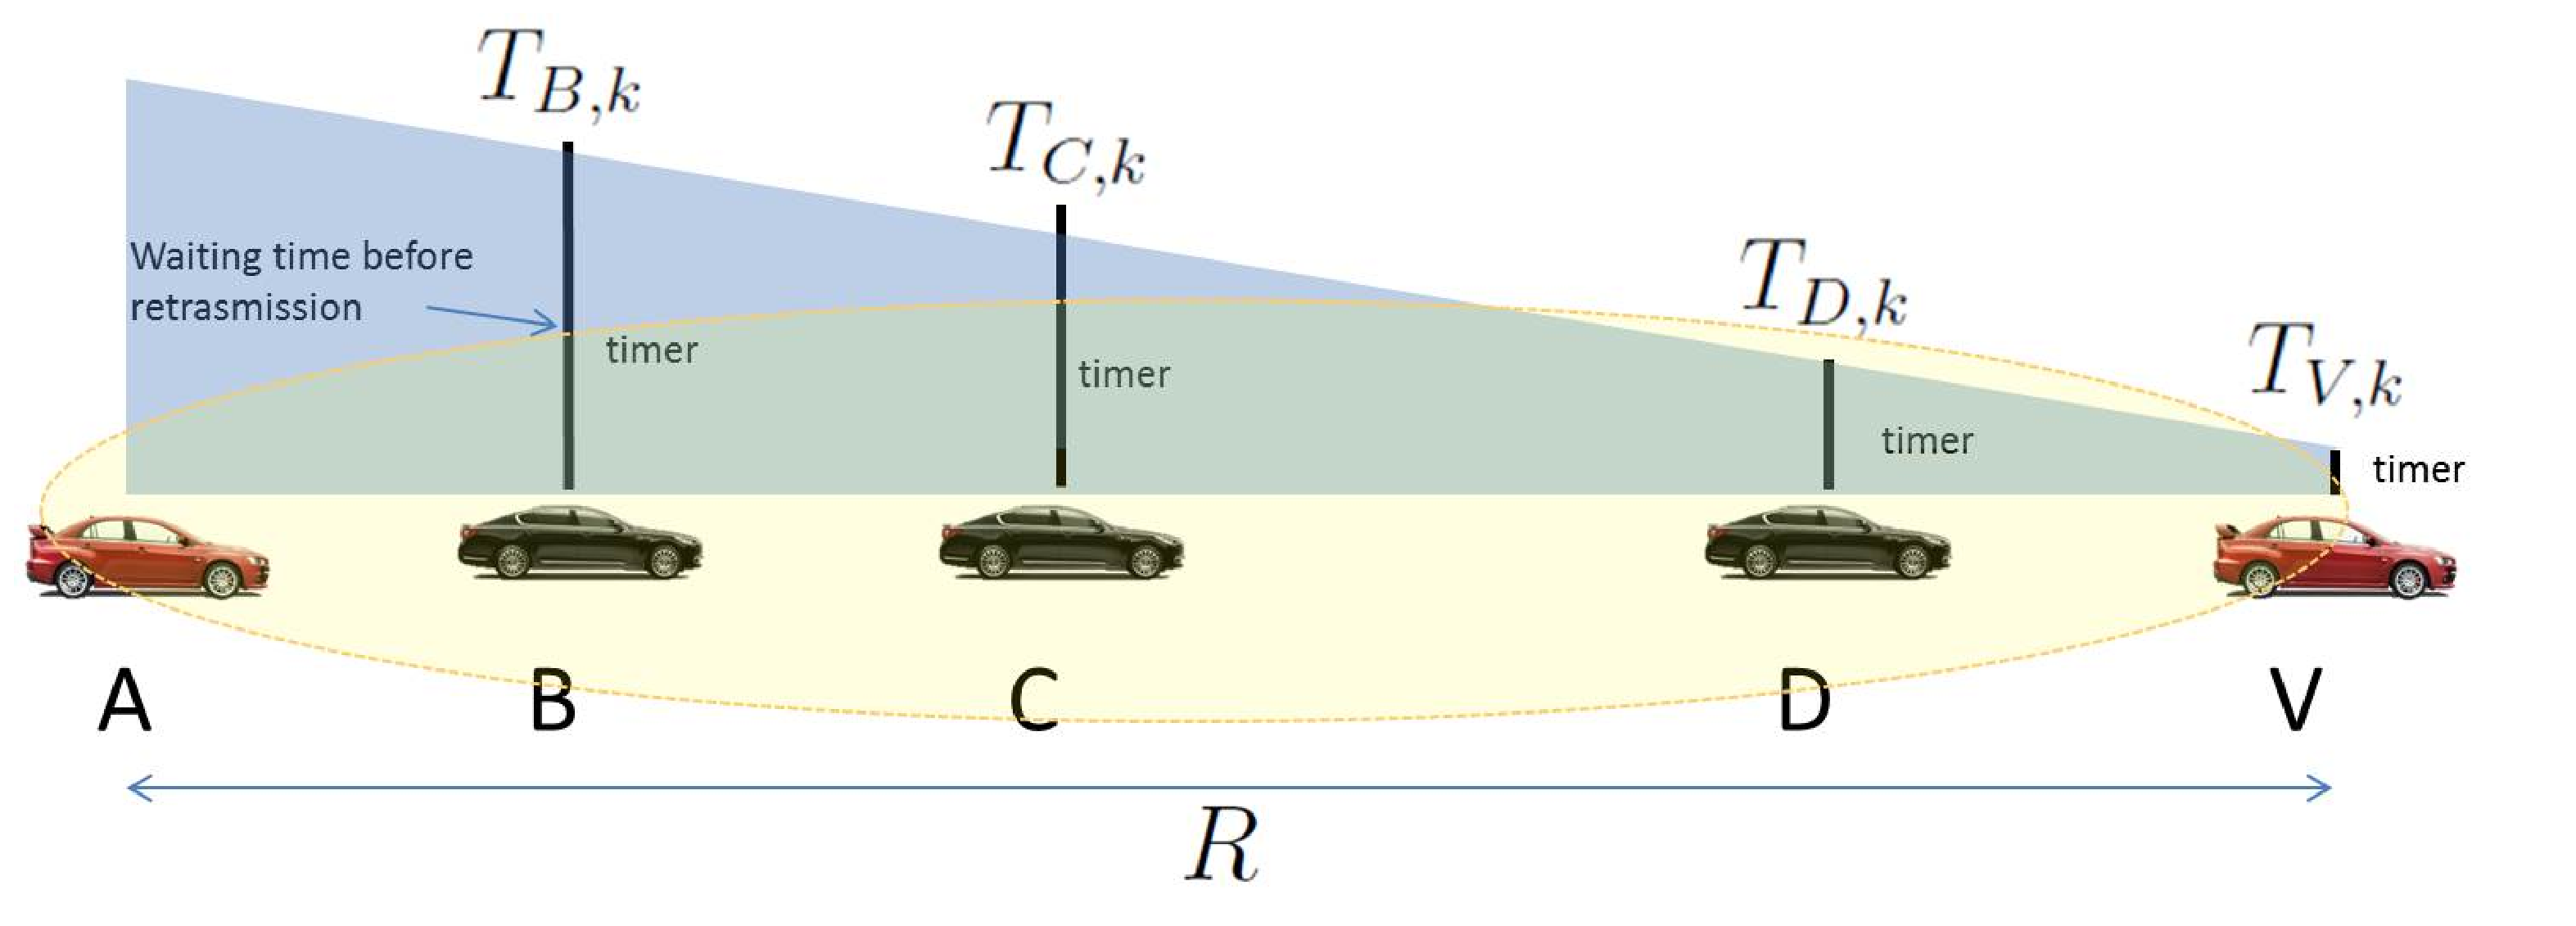
\includegraphics[width=0.8\columnwidth]{fig/SAME.eps}
\caption{DBF retransmission logic based on timers (black bars) inversely proportional to the distance form the sender. Oval box represents the maximum transmission range $R$ of sender $A$.}
\label{fig:same}
\end{center}
\end{figure}


\begin{figure*}[tbhp]
\begin{center}
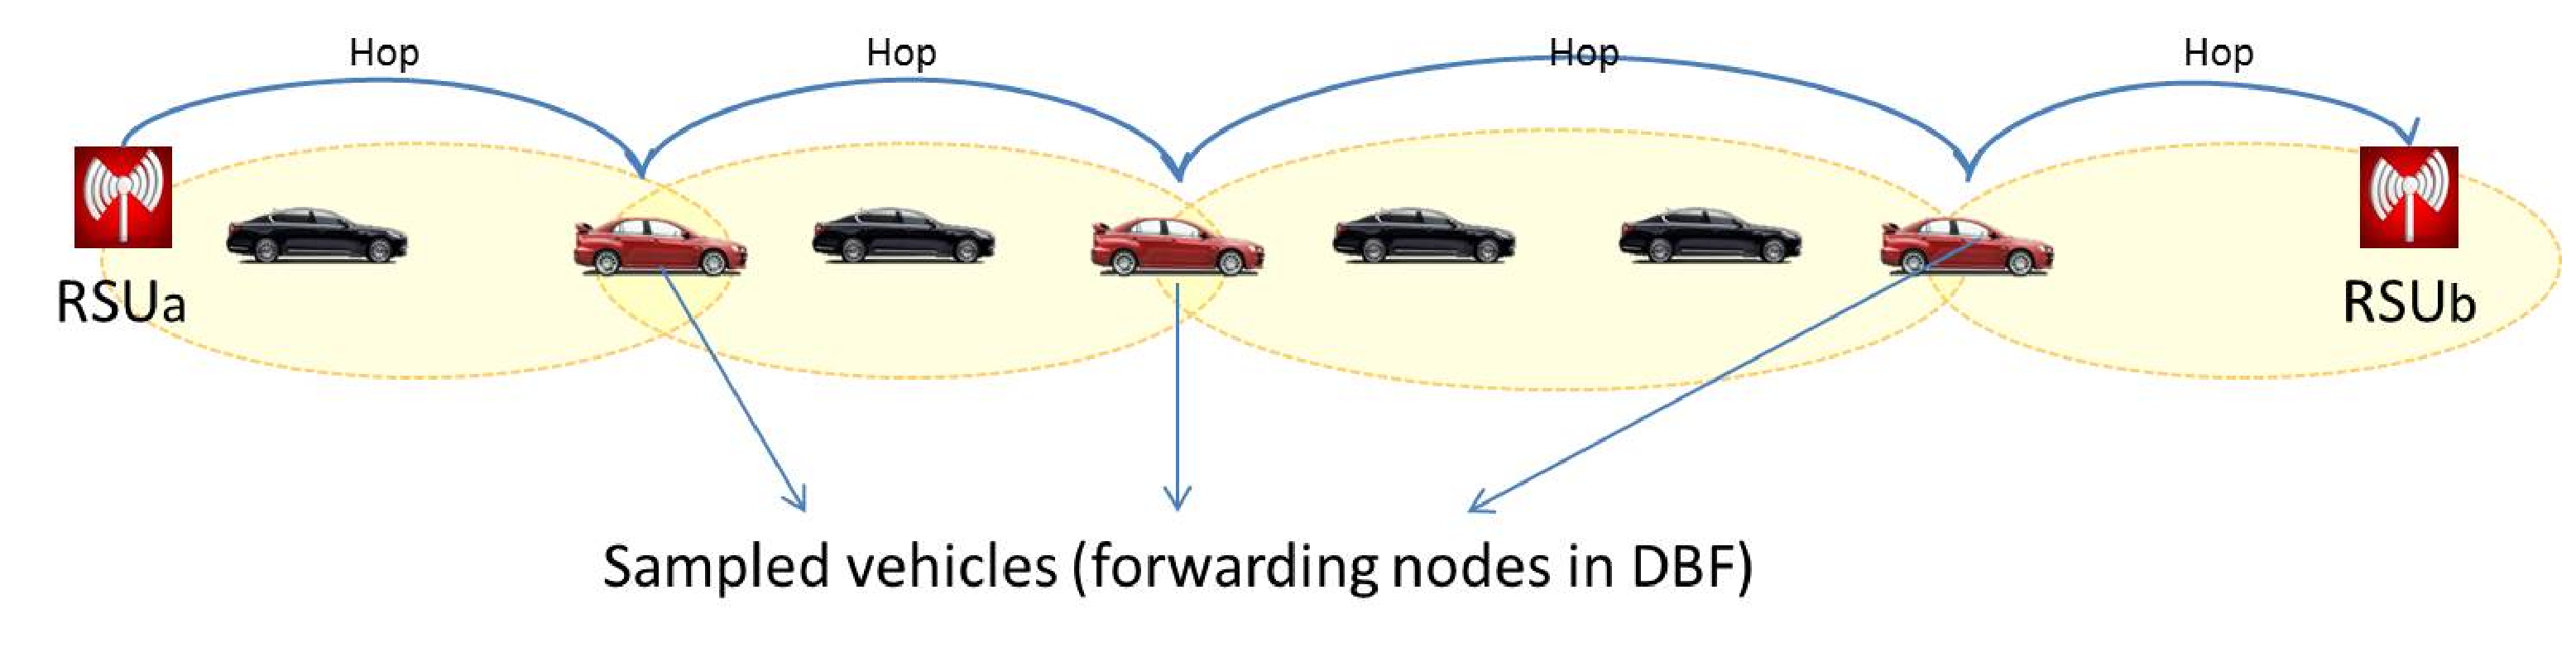
\includegraphics[width=1.8\columnwidth]{fig/SAME_HOP.eps}
\caption{An example of multi-hopping in the SAME logic from $\text{RSU}_a$ to $\text{RSU}_b$. Only red cars are the sampled vehicles. Oval boxes represent maximum transmission ranges.}
\label{fig:same_hop}
\end{center}
\end{figure*}



The logic defined to monitor the traffic on the road with the VANET is implemented by having a distributed collection of a vector $\mathbf m = (m_1,\ldots,m_n)$ where the $i$th element is a 4-tuple $m_i=\langle P_i, v_i, d_i, t_i \rangle$. Here $P_i$ contains the geographical coordinates of the $i$-th sampled vehicle, $v_i$ contains its current speed and $d_i$ the direction,  $t_i$ is a timestamp with the current time. The size of $\mathbf m$ depends on the number of vehicles that collect this information, that is the number of vehicles forwarding the message (or the number of hops) from the source RSU up to the sink RSU. The message initially issued by $\text{RSU}_a$ has an empty payload. Each sampled vehicle, namely a vehicle acting as a forwarding node according to DBF, appends its 3-tuple to the current payload of the message. When the message reaches $\text{RSU}_b$, it carries all $n$ collected measurements. $n$ is related to the average hop length and to the length of the monitored road span. A fast polling is possible, since each forwarding hop takes a time in the order of ms and typical hop lengths can be several hundred meters. The traveling speed of the monitoring messages can be thus in the order of 50~km/s, three orders of magnitude more than vehicle speed. Measurements are collected at the $\text{RSU}_b$ and can be used to track the traffic average speed and density in each sector of the monitored road span. Polling is repeated every $\tau_{RSU}$ seconds. $\tau_{RSU}$ is to be chosen so as to detect vehicular traffic variations quickly and reliably (that entails collecting tens of samples over a time scale comparable with that of vehicle motion, namely minutes) and to keep the collecting protocol performance near to optimal by avoiding communication channel congestion (which implies taking $\tau_{RSU} \gg \tau_{prop}$, where $\tau_{prop}$ is the time required for the message to travel a distance much bigger than the transmission range of a OBU; it is enough to take $\tau_{RSU}$ in the order of seconds).


\subsection{Exhaustive measurement collection logic - TOME}
\label{subsec:DBFexh}
DBF and similar multi-hopping protocols lend themselves naturally to sampled measurement collection, where samples are taken according to the distance covered at each hop. An exhaustive collection of vehicle measurements can be achieved by devising a variation of such protocol; the biggest difference is that all vehicles are assumed to send their own message, instead of having only a selection of relaying vehicles that forward the measurement message. We propose the Timer-based Ordered Measurement Estimation (TOME) protocol.


The protocol is based on an initiator station, namely an RSU, polling the system with $cmc$ messages with period $\tau_{RSU}$. $\tau_{RSU}$ is much bigger than the single hop time, so as to avoid MAC level congestion. The Collection Road Segment (CRS) is defined as the span of road for which the protocol aims at giving a single estimate of the average speed and density of vehicles. Let $d_0$ denote the target CRS length. For each CRS a node plays the role of the CRS Initiator (CRSI), i.e., it resets the message accumulator fields and starts off a new CRS.

Messages are made up of three parts: i) a header, that lists the sequence number $k$, the identity of the sending node $S$ and its position $P_S$; ii) the list $\mathcal{L}$ of the measurements consolidated from previous CRSs; iii) the current CRS record $\langle CRSI.id,CRSI.pos,AS,NV \rangle$. $CRSI.id$ and $CRSI.pos$ are the CRSI identity and position of the vehicle playing the role of initiator of the CRS. $AS$ is an accumulator field, whose value is the current sum of the speeds of vehicles that have been passing the message to one another within the CRS. $NV$ is an integer counter, carrying the number of vehicles that have contributed to the accumulator $AS$. We denote formally a message as $\mathcal{M}=[k,S,P_S;\mathcal{L};\langle CRSI.id,CRSI.pos,AS,NV \rangle]$.

At the end of the CRS $s$, the attained values $AS_s$ and $NV_s$ are frozen and stored into the list, i.e., $\mathcal{L}=\mathcal{L} || \langle P_{s}, AS_s,NV_s \rangle$, where $P_{s}$ is the position of the first node of CRS $s$. The notation $||$ means appending the record appearing on the right to the list denoted at the left of the sign. The consolidation of the record appended to the list is done by the node that starts the new CRS $s+1$, namely the node in position $P_{s+1}$.

Each node maintains state variables. For node $A$ we define:
\begin{itemize}
 \item $k_A$, the biggest sequence number read from incoming messages;
  \item the current measurement tuple $\mathcal{T}_A=\langle CRSI.id_A,CRSI.pos_A,AS_A,NV_A \rangle$, as updated after the reception of the most recent relevant TOME protocol message;
  \item $T{A, k}$ the current value of the timer of $A$ as for the $k$th message.
  \end{itemize}

The basic idea of TOME is that each vehicle receiving a collection message will schedule the emission of its own message copy. The copy includes any accumulated speed sum heard of until emission time, plus the contribution of the vehicle's own speed. The only exception is when a vehicle deems to be a new CRSI. In that case the most recent contribution, received before the scheduled emission time, is frozen into the list and a new accumulation starts off.

An example of the operation of TOME is given in Figure \ref{fig:tome}. Vehicle $A$ is the CRSI, timers are highlighted as vertical bars. The black part of the bar represents the timer duration. Every vehicle in the CRS has its transmission range $R$ ($R_A$, $R_B$ and $R_C$ in the figure). All vehicles in the CRS send their measurements.

\begin{figure}[tbhp]
\begin{center}
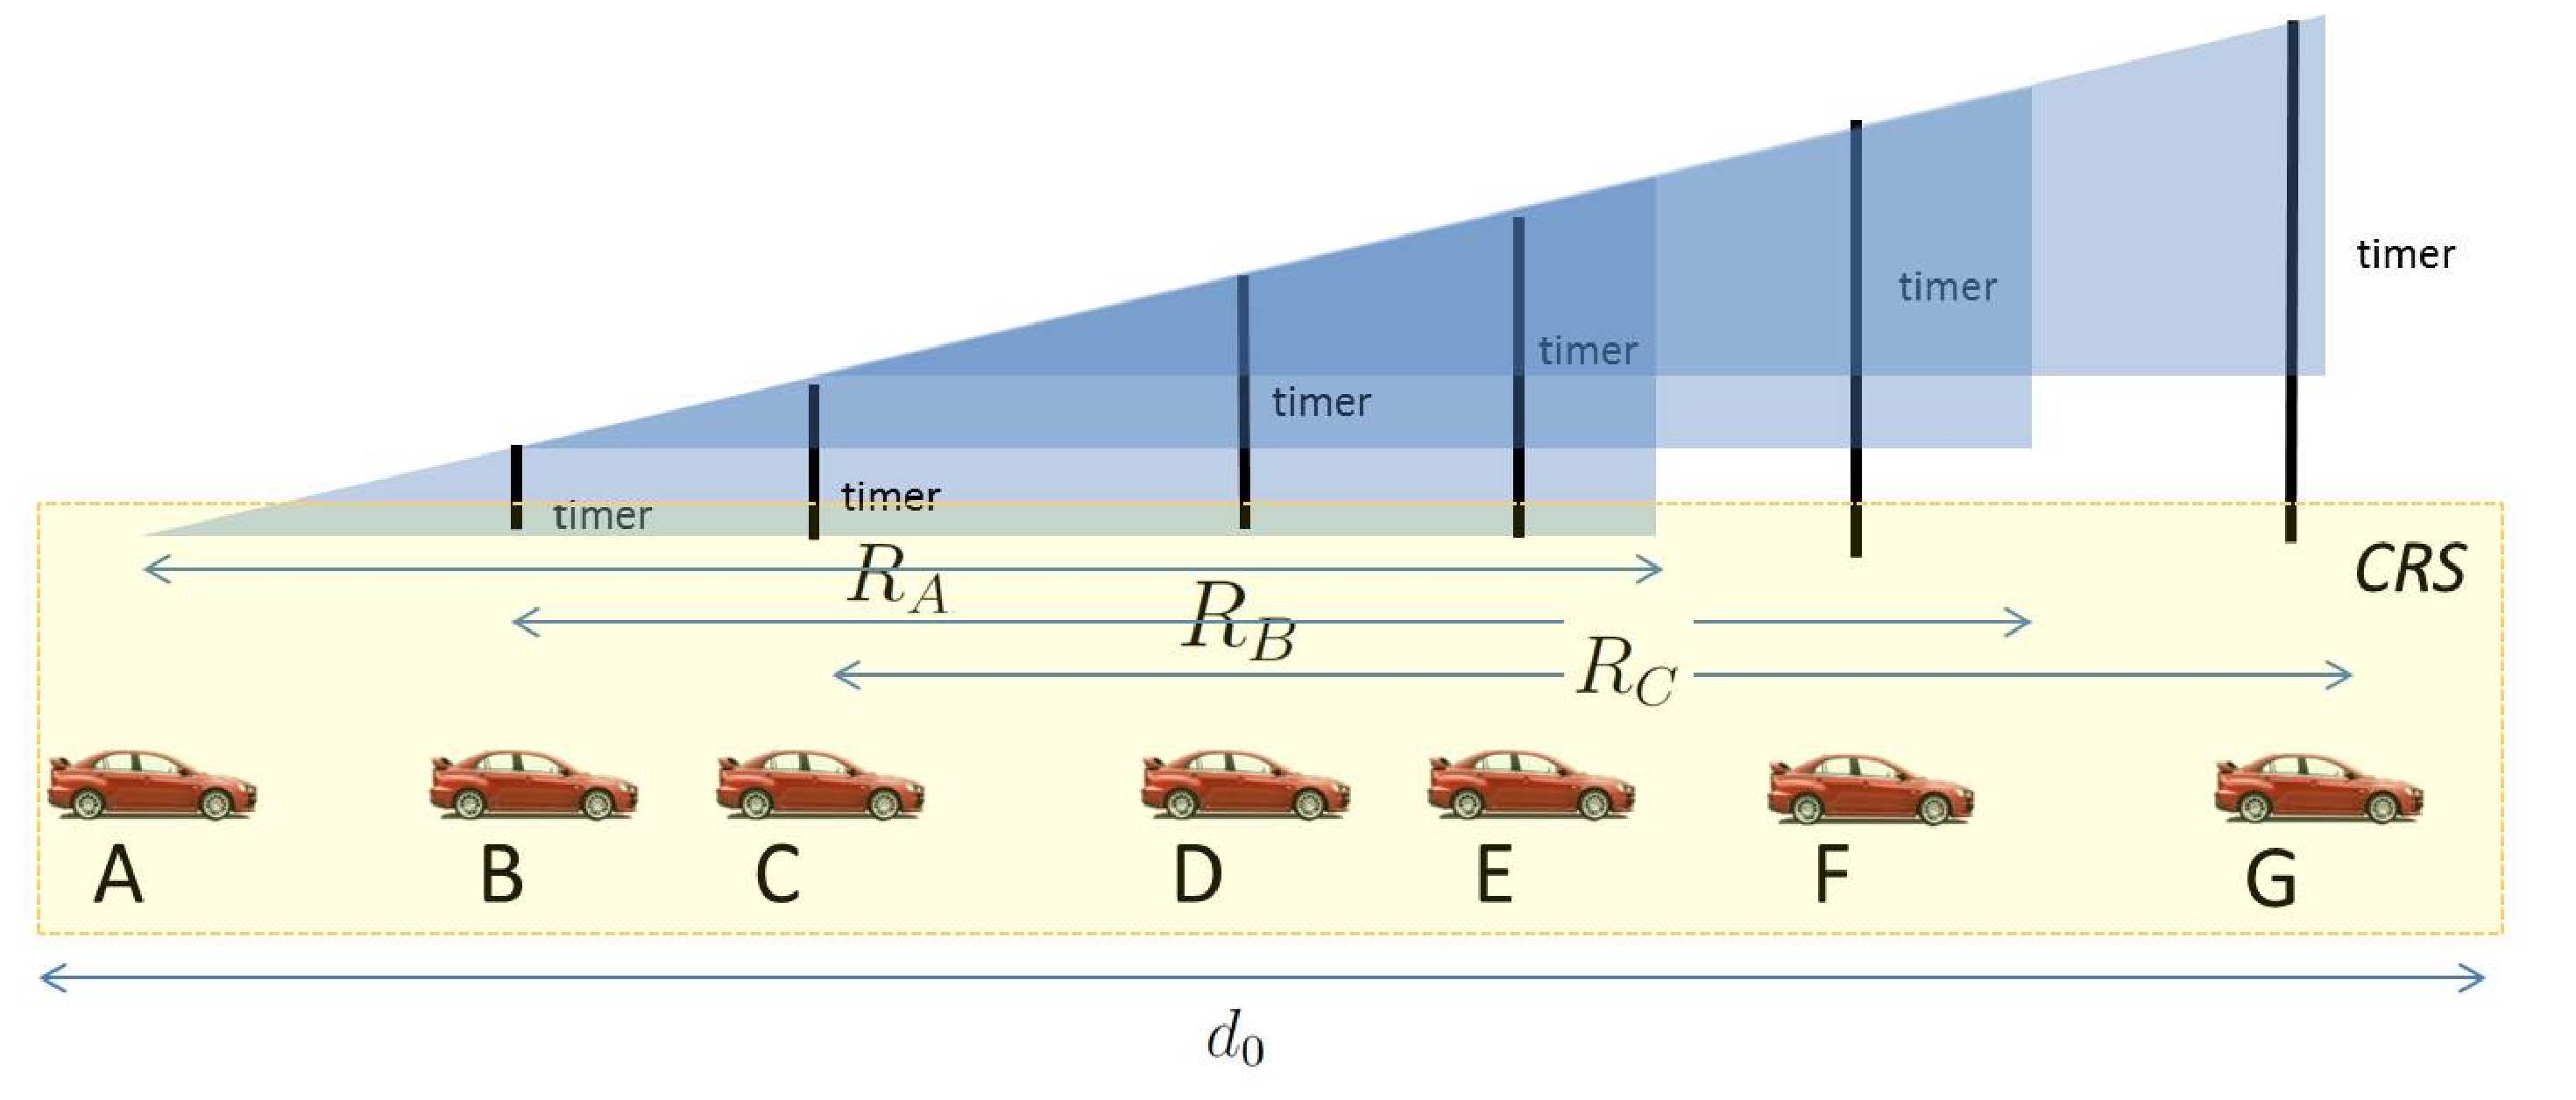
\includegraphics[width=0.8\columnwidth]{fig/TOME.eps}
\caption{An example of data collection in case of TOME over one Collection Road Segment. Retransmission timers are directly proportional to the distance. The rectangular box represents the CSI.}
\label{fig:tome}
\end{center}
\end{figure}

It can be noted that timer values are kept as chosen when receiving the first message with a new sequence number. Subsequent messages with the same sequence number do not cause the timer to be updated. This leads to \emph{ordered termination of the timers} according to the distance from the CRSI. This property stems from the monotone rule chosen to set the initial values of timers, according to the distance of the receiving node from the CRSI. For each CRS, the RSU receives at last the collected sum of speeds $V$ in the segment and the overall number of vehicles $N$, hence it can estimate the average speed ($V/N$) and the average vehicle density as $\delta=N/d_0$. Given $V$ and $\delta$, the average flow of the MCS is derived as $\phi = V \delta$.

Let us consider a node $B$ with state $k_B$ and $\mathcal{T}_B = \langle X,P_X,v,n \rangle$, when it receives the message $\mathcal{M}=[k,A,P_A|\mathcal{L}|\langle Y,P_Y,V,N \rangle]$.
% In the following we denote the distance between two node positions $P$ and $Q$ as $\overline{PQ}$.

If $k < k_B$, the new message is ignored, as an old, out of date message.

If $k = k_B$, $B$ checks if $Y=X$. In that case, $B$ has received a message from a vehicle inside the same CRS as $B$ is. So, if $N>n$, $B$ updates its state as follows: $\mathcal{T}_B \leftarrow \langle X,P_X,V,N \rangle$ and reschedules its timer as $T_{B,k}=T_{max}\overline{P_AP_B}/R_{max}$. If instead it is $N \le n$, $B$ does nothing and ignores the received message.

If $k = k_B$, but it is $Y \ne X$, then $B$ checks whether $\overline{P_YP_B}<\overline{P_XP_A}$ and $\overline{P_YP_X}<\overline{P_XP_B}$. In that case $B$ reassigns itself to the CRS initiated by $Y$ and updates its tuple to  $\mathcal{T}_B=\langle Y,P_Y,V,N \rangle$ and timer to $T_{B,k}=T_{max}\overline{P_AP_B}/R_{max}$. In case it is found that $\overline{P_YP_B} \ge \overline{P_XP_B}$ or $\overline{P_YP_X} \ge \overline{P_XP_A}$, $B$ does nothing and ignores the message.

If $k > k_B$, a new measurement cycle is being run and $B$ updates its state as $k_B=k$. As for the tuple $\mathcal{T}_B$, the key point is to check whether $B$ has to start a new CRS or it belongs to the current CRS. Hence $B$ checks if $\overline{P_YP_B} > d_0$. In that case, $B$ sets $\mathcal{T}_B=\langle B,P_B,0,0 \rangle$. If instead it is $\overline{P_YP_B} \le d_0$, $B$ sets $\mathcal{T}_B=\langle Y,P_Y,V,N \rangle$. In any case, a countdown timer is started with the initial value $T_{B,k}=T_{max}\overline{P_AP_B}/R_{max}$.

Finally, when the timer $T_{B,k}$ expires and the state of $B$ is $k_B$ and $\langle X,P_X,v,n \rangle$, $B$ sends out a message $\mathcal{M}=[ k_B,B,P_B|\mathcal{L}|\langle X,P_X,v+v_B,n+1 \rangle ]$, where $v_B$ is the current speed of $B$.

An example of TOME behavior over multiple CRSs is given in Figure \ref{fig:tome_hop}. When the CRSI of CRS1 sends the message ($A$ in this case) all nodes with a distance $\overline{P_YP_B} \le d_0$ will retransmit the message by adding their speed values and positions. On the contrary when a node is out of the CRS ($H$ in the example) it re-elects itself as CRSI, updates the list of other CRSs with the last measurements arrived and starts a new measurements collection over the new segment. The result is that for CRS1 the averaged speed value is over 7 vehicles while for CRS2 over 4 cars.

\begin{figure*}[tbhp]
\begin{center}
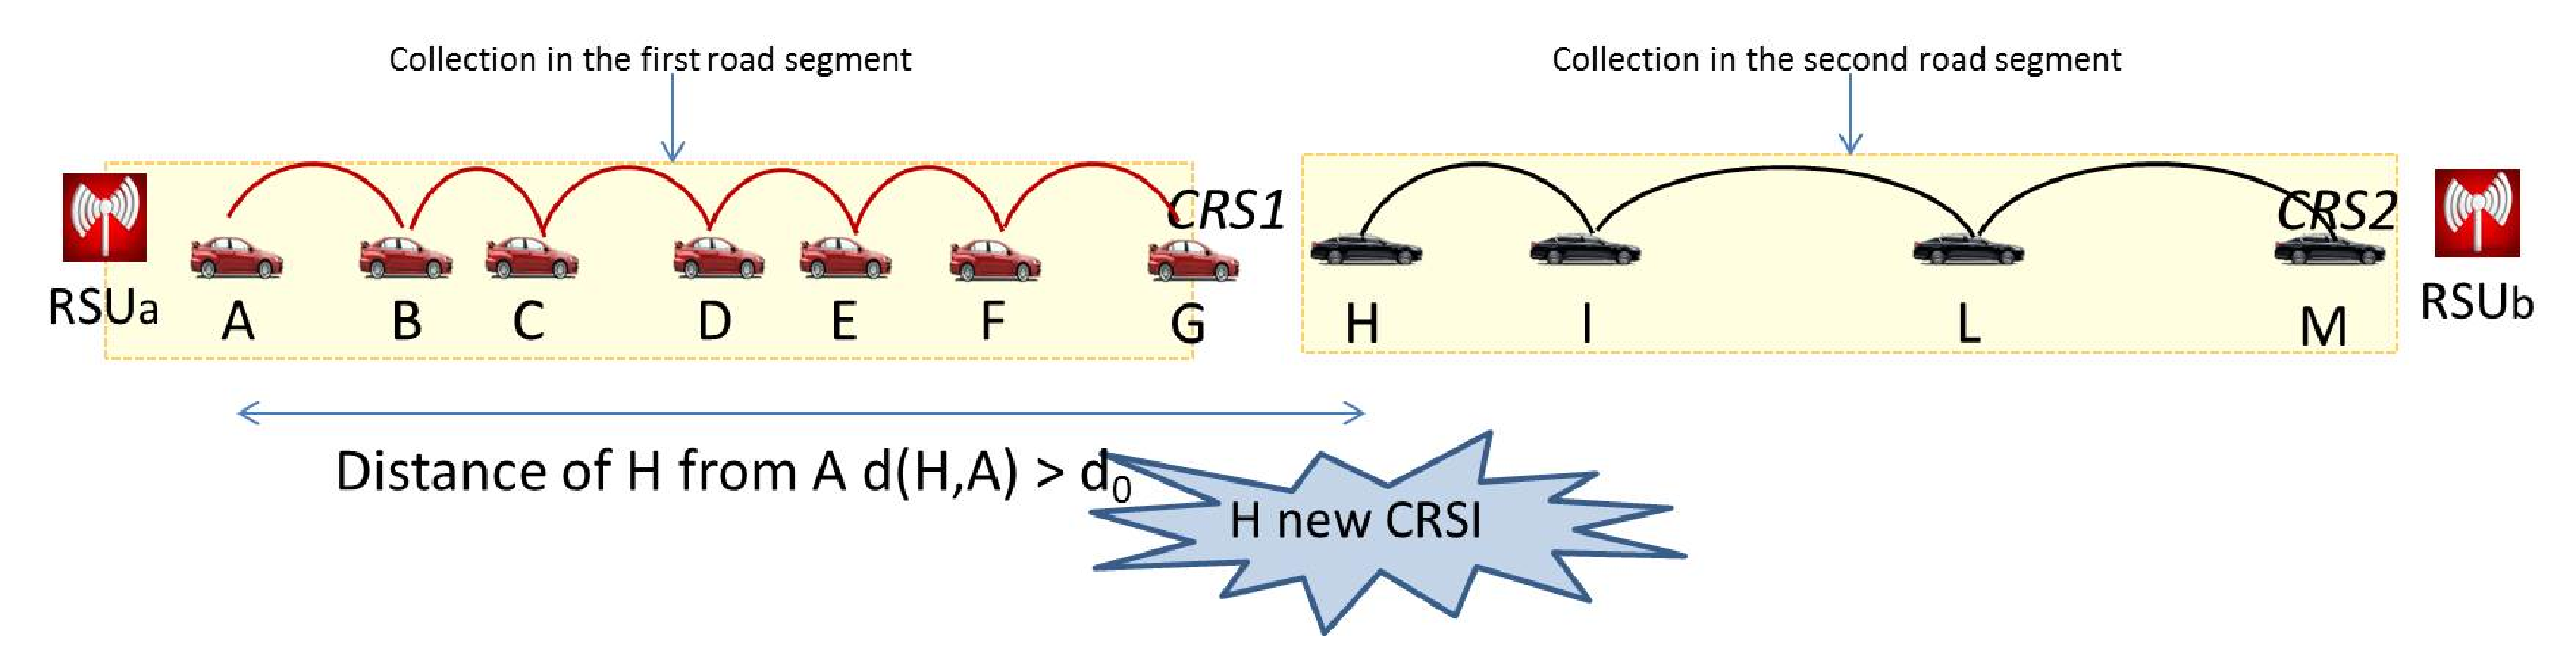
\includegraphics[width=1.8\columnwidth]{fig/TOME_HOP.eps}
\caption{TOME behavior over two CRSs. CSRI in the first segment is $A$ while in the second segment is $H$.}
\label{fig:tome_hop}
\end{center}
\end{figure*}


The speed of propagation of the measurement collection message is $R/T_{max}$. For typical values of the involved parameters, the order of magnitude of this speed is tens of thousands of km/h, so that it is from two to three orders of magnitude bigger than vehicle speed. As a matter of example, with $T_{max}=500~ms$, $R_{max}=830~m$, to cover the GRA (about $68~km$), it takes about $41~sec$.

As for the size of the measurement collection message, we assume that a position can be represented with 16 bits, the accumulated average speed as a floating number with 32 bits and the number of vehicles per segment as a 16 bit integer. Then 80 bits = 10 bytes are sufficient for a single record of the list. The number of MCSs depends on $d_0$ and the length $L$ of the observed road, namely it is $\lceil L/d_0 \rceil$. If the measurement collection process involves no more than 100 road segments, 1000 bytes are enough to hold the whole list. Therefore, it can be expected that the message length is at most somewhat more than 1000 bytes, which is well compatible with message sizes sent over the DSRC interface.

Structures of the messages propagated in case of SOME and TOME are reported in Figure \ref{fig:mess}. In case of TOME the message is the one crossing the second CRS and transmitted by the node $I$; $H$ is the CRSI of this second segment while the CRSI of the first segment is $A$.


\begin{figure*}[tbhp]
\begin{center}
\includegraphics[width=1.8\columnwidth]{fig/message.eps}
\caption{Messages propagated in case of SOME and TOME.}
\label{fig:mess}
\end{center}
\end{figure*}


\section{Application of monitoring protocols to a urban highway}
\label{sec:realcase}
In order to set up a realistic simulation, we exploit a large database of about 104 millions of GPS traces collected by about 80,000 equipped vehicles that made about 9 millions trips during the month of May 2010 in the metropolitan area of Roma (Italy). We focused on a subset of 50,220 vehicles on a 68~km long ring-shaped expressway embracing the city called GRA, which collects and distributes long-haul traffic entering and exiting from the city (see Fig. \ref{fig:scenario}). Each vehicle sends its information record every 30 seconds. A variety of information is provided by each record, including the vehicle ID, geographical coordinates, speed and quality of GPS signal. Our FCD (Floating Car Data) has been cleaned of the records with low GPS signal quality in order to consider only highly reliable data.

\begin{figure}[tb]
\begin{center}
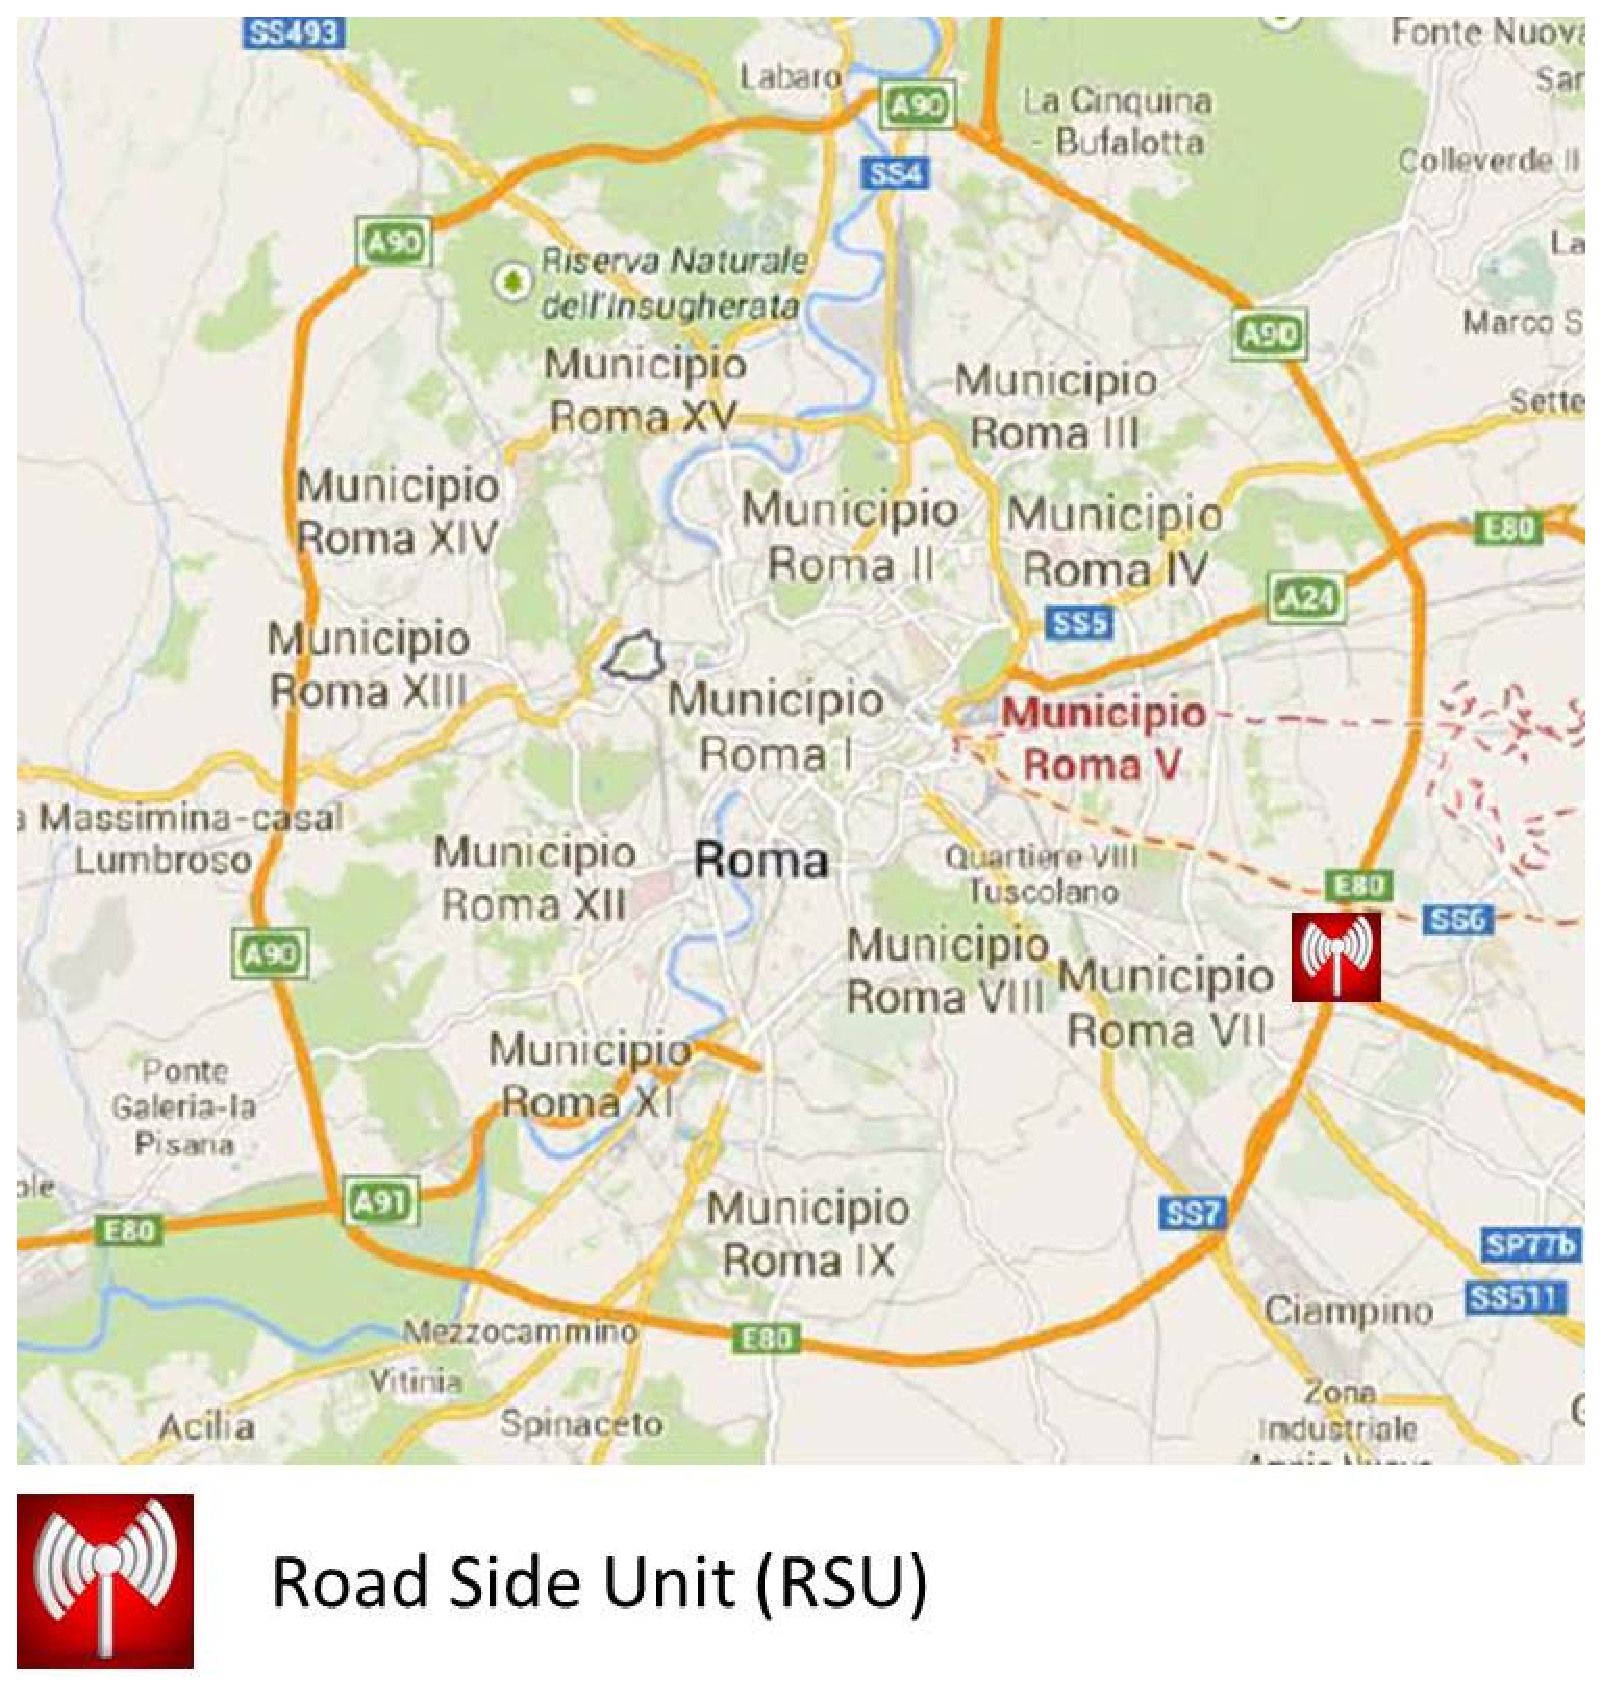
\includegraphics[width=.8\columnwidth]{fig/Scenario.eps}
\caption{The scenario we are working on. The RSU is highlighted in red}
\label{fig:scenario}
\end{center}
\end{figure}

In order to analyse the data, we have divided the GRA in 29 different segments of length $L_j$, $j=1,\dots, 29$, where the main exits from the GRA highway are the starting and ending points of each segment. Vehicles were then divided in two sets according to their traffic direction: clockwise and counterclockwise. Four different time periods of four hours each have been considered, starting from 7~am until 11~pm. Inter-vehicle distance distribution and speed distribution were obtained  for each of the four time periods. This analysis showed that the highest density of vehicles is in the time period between 3~pm and 7~pm, which has the largest number of detected vehicles (9732 vehicles).

To set up a realistic mobility simulation of the urban traffic on the GRA, the available data sample have been inferred to the universe of vehicles by assuming a random uniform sampling. Let $\Delta t$ be the sampling interval ($30~sec$ in our study), $v_i$ the average speed of vehicle $i$, $n_j$ the estimated number of vehicles traveling in the $j$-th segment, $g_j(t_1,t_2)$ the number of detected GPS signals in the $j$-th segment during the observation time interval $[t_1,t_2]$, $L_j$ the length of the $j$-th segment, $a$ the probe vehicles penetration rate ($a \approx 2.3\%$ in our study) and $q_j$ the estimated flow on the $j$-th segment. Then: %$n_j=\sum_{i=1}^{g_j(t_1,t_2)} \frac{ v_i \Delta t}{L_j}$ and the resulting flow is $q_j = \frac{n_j}{a(t_2-t_1)}$.
\begin{equation}
n_j=\sum_{i=1}^{g_j(t_1,t_2)} \frac{ v_i \Delta t}{L_j}
\end{equation}
and the resulting flow is $q_j = \frac{n_j}{a(t_2-t_1)}$. The above inference relations have been applied to the traffic flows in the peak period and have been used to enter into each segment $j$ a flow of vehicles of mean intensity $q_j$. The FCD have been used to estimate the OD matrix, where Origins and Destinations correspond to the exits of GRA. Vehicle attributes have been tuned so that the average speed values measured per lane and per segment with the mobility simulation software match the corresponding values estimated with the inferred experimental data.




%\begin{figure*}[!t]
%\begin{center}
%\subfigure[penetration level 1]{\label{fig:incid_pen1}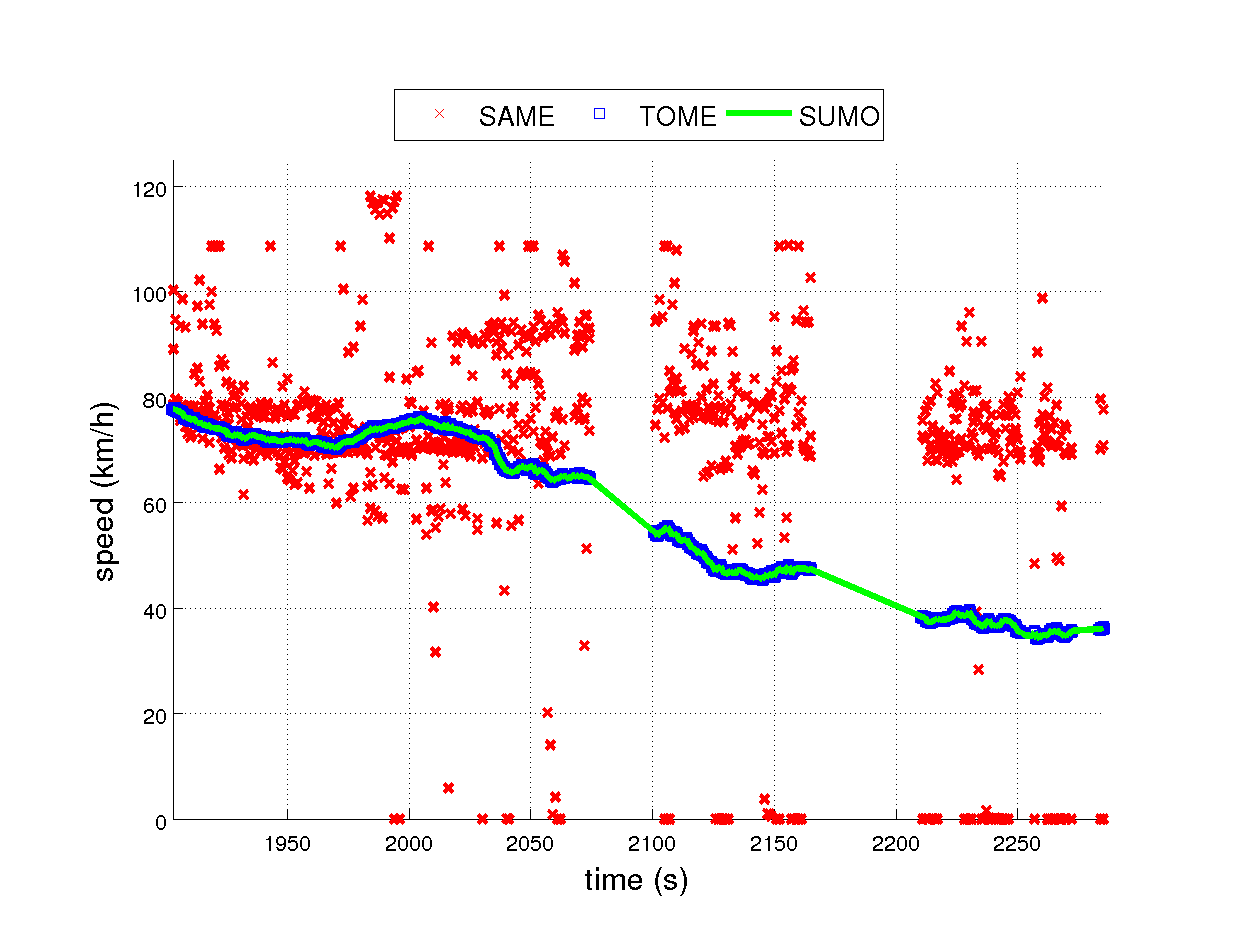
\includegraphics[width=.65\columnwidth]{fig/penetration_incidente_sett141.eps}}
%\subfigure[penetration level 0.75]{\label{fig:incid_pen075}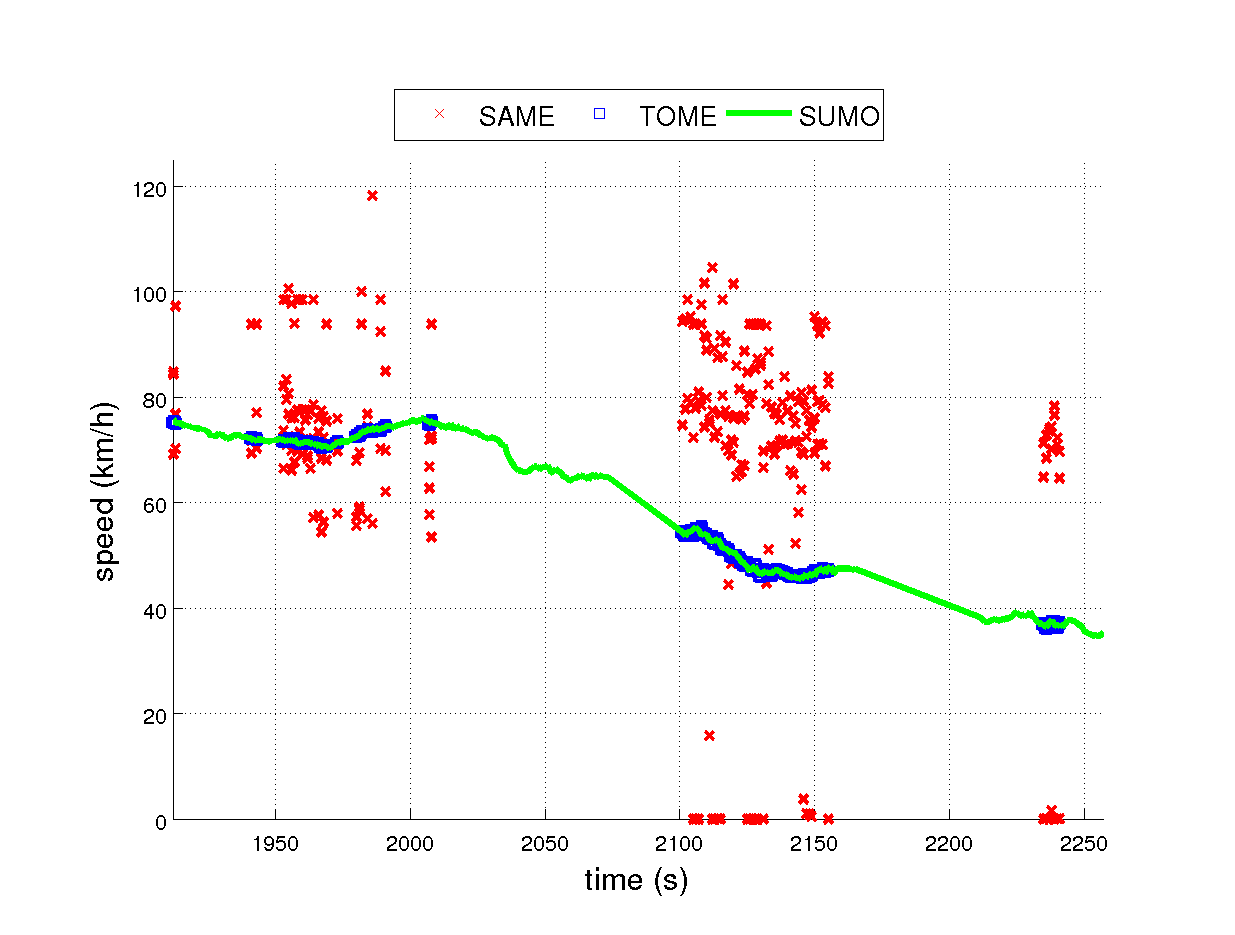
\includegraphics[width=.65\columnwidth]{fig/penetration_incidente_sett140.75.eps}}
%\subfigure[penetration level 0.5]{\label{fig:incid_pen05}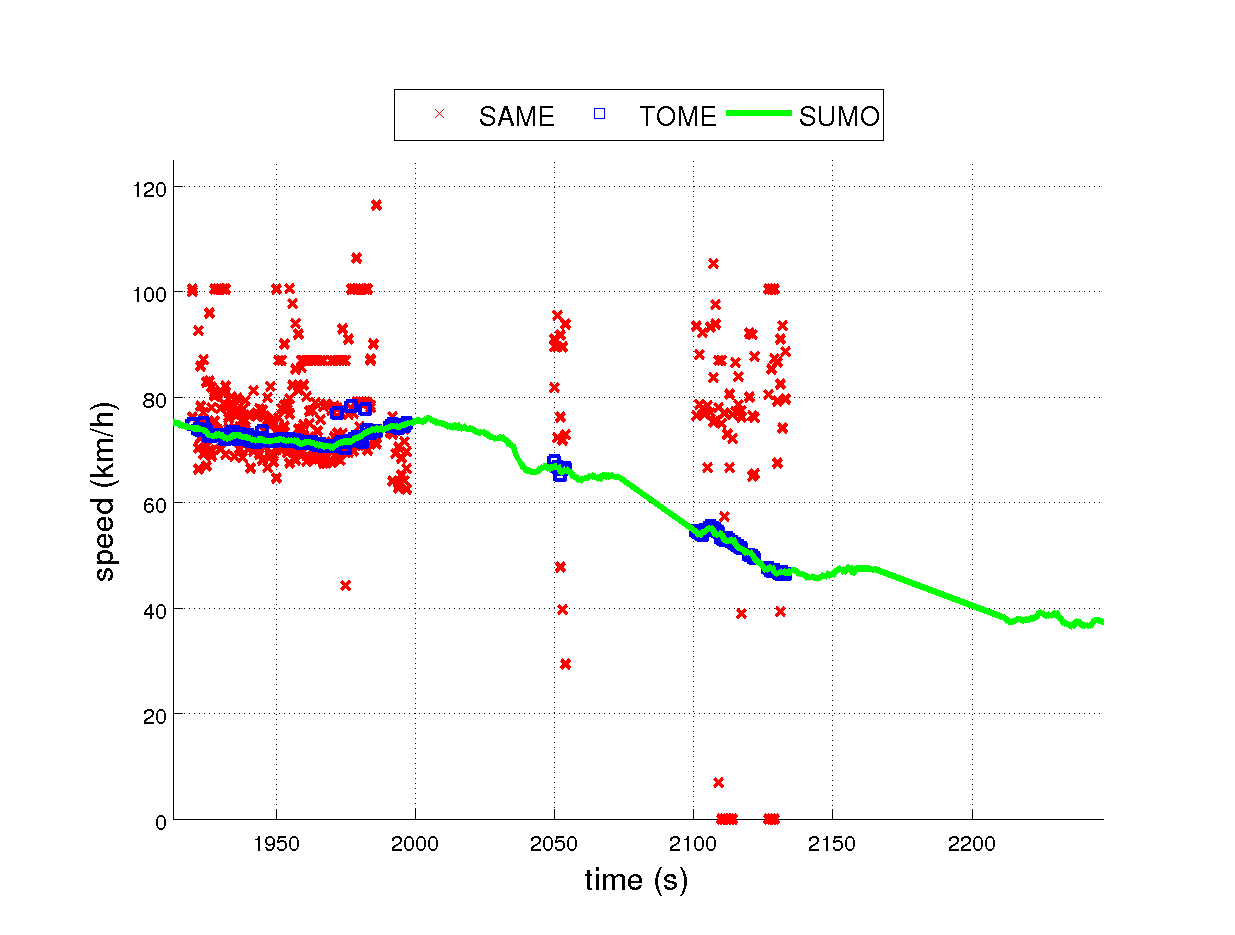
\includegraphics[width=.65\columnwidth]{fig/penetration_incidente_sett140.5.eps}}
%\caption{Speed measure when varying the penetration rate of our system in case of incident}
%\label{fig:penetration_incidente}
%\end{center}
%\end{figure*}


\section{Performance Evaluation}
\label{performance}

\subsection{Simulation model}

%spiegazione simulatori
%come sono state fatte le varie simulazioni, spiega penetration rate, durata sim, etc creaz incidente
%tabella simulatore
%come sono ottenuti i grafici ? Qui o dopo in perf analysis ?

For our case study of urban highway, we have imported the map of the Rome GRA from Open Street Map \cite{openstreetmap} to SUMO \cite{SUMO}, where we have generated and verified the traffic flows from our OD matrix analysis in Section \ref{sec:realcase}. We have implemented our VANET monitoring logics, as described in Section \ref{sec:monitoring}), by adding code to NS2 \cite{ns2} to realise the Forwarding Layer protocols on top of the IEEE 802.11p MAC/PHY layers already built in NS2. Communication network simulations of NS2 are fed by the outcome of SUMO to give node positions, sampled once per second. Between two consecutive sampling times, NS2 moves nodes according to linear uniform motion.

Since it will take years to deploy the VANET technology extensively, we assume different market penetration percentages of VANET DSRC radio equipment on board vehicles. Because of this, every new vehicle that is instantiated in our simulations, is equipped with this technology with probability $p \in [0,1]$, that represents the market penetration rate of the VANET technology. So, on average, only $p\cdot 100\%$ of the vehicles are able to communicate with each other, while the others do not perform any transmission/reception operation, although influencing the vehicular micro-mobility simulated by SUMO.

We set up two simulation scenarios: i) regular traffic conditions, as given in the peak period identified in Section \ref{sec:realcase}, based on the collected FCD on Rome GRA; ii) incident scenario. In the latter one, the flows are as in the regualar  scenario, except that in a specific highway sector (\#14), just before time $t=2000~sec$, we raised the speed of some vehicles (the dense high speed cloud in Fig. \ref{fig:incid_pen1}) thus ending up with a car incident that obstructs two out of the three lanes of the road in the considered traveling direction, until the end of the simulation.

Tab. \ref{tab:parameters} lists the main simulation parameters.

\begin{table}[t]
	\caption{Simulation parameter values}
	\label{tab:parameters}
	\centering
\small
	\begin{tabular}{l|l}
		\hline
		\multicolumn{1}{l|}{\textbf{Parameter}} & \multicolumn{1}{l}{\textbf{Value}} \\
		\hline
		Road length (km) & 68.2 \\
		Number of lanes per traveling direction & 3 \\
		Average vehicle density (veh/km) & $31.02$ \\
		SUMO simulation duration (s) & 3600 \\
		Network simulation duration (s) & 350-400s \\
		Frequency of generated messages (msg/s) & 1  \\
		%Transmission Power (mW) & 500 \\
		$R_{max}$ for each tx power value (m) & 827 \\
		Max forwarding delay, $T_{max}$ (ms) & $100$\\
		Link Rate (Mbit/s) & $6$\\
		MAC, PHY parameters & IEEE 802.11p \\
		Propagation Model & Two ray ground \\
		\hline
	\end{tabular}
\end{table}

%important to make a graphic, like the one that prof. Fusco prepared for Dresden presentation, which is unpublished (see Figure \ref{fig:reliability}). The problem is that now we have a new SUMO version that allows the tuning of brand new parameters, so we have different outcomes and trends.
%We can then focus on penetration rates.
%Most of the times the sampled speed is higher than the real one. Since the frequency of the faster vehicles is higher than the one of the slower ones, then it is more likely to sample the ones that travel faster.


\subsection{Traffic monitoring in regular conditions}
\label{subsec:stationary}
We assume regular traffic conditions on the considered urban highway and we feed vehicular traffic according to the statistics derived from measurements in the peak time interval, as explained in Section \ref{sec:realcase}. A single RSU is placed as shown in Figure \ref{fig:scenario} and it acts contemporarily as $cmc$ originator and sink. It sends out $cmc$ with a time period $\tau_{RSU}=1~sec$.
%fig:incid_pen1
Figure \ref{fig:pen1}, \ref{fig:pen075} and \ref{fig:pen05} plot the average speed measured over the entire urban highway through SAME and TOME and as given by the simulation software SUMO (ground truth). Measurements arriving at the RSU after taking a full trip along the urban highway ring are averaged out over a time window of $5~sec$ (on top) and $1~sec$ (bottom). The three graphics assume different fractions of vehicles equipped with a VANET OBU, namely $p=1$, $0.75$ and $0.5$.


\begin{figure*}[tbhp]
\begin{center}
\subfigure[100\% of OBU-equipped vehicles, regular traffic conditions]{\label{fig:pen1}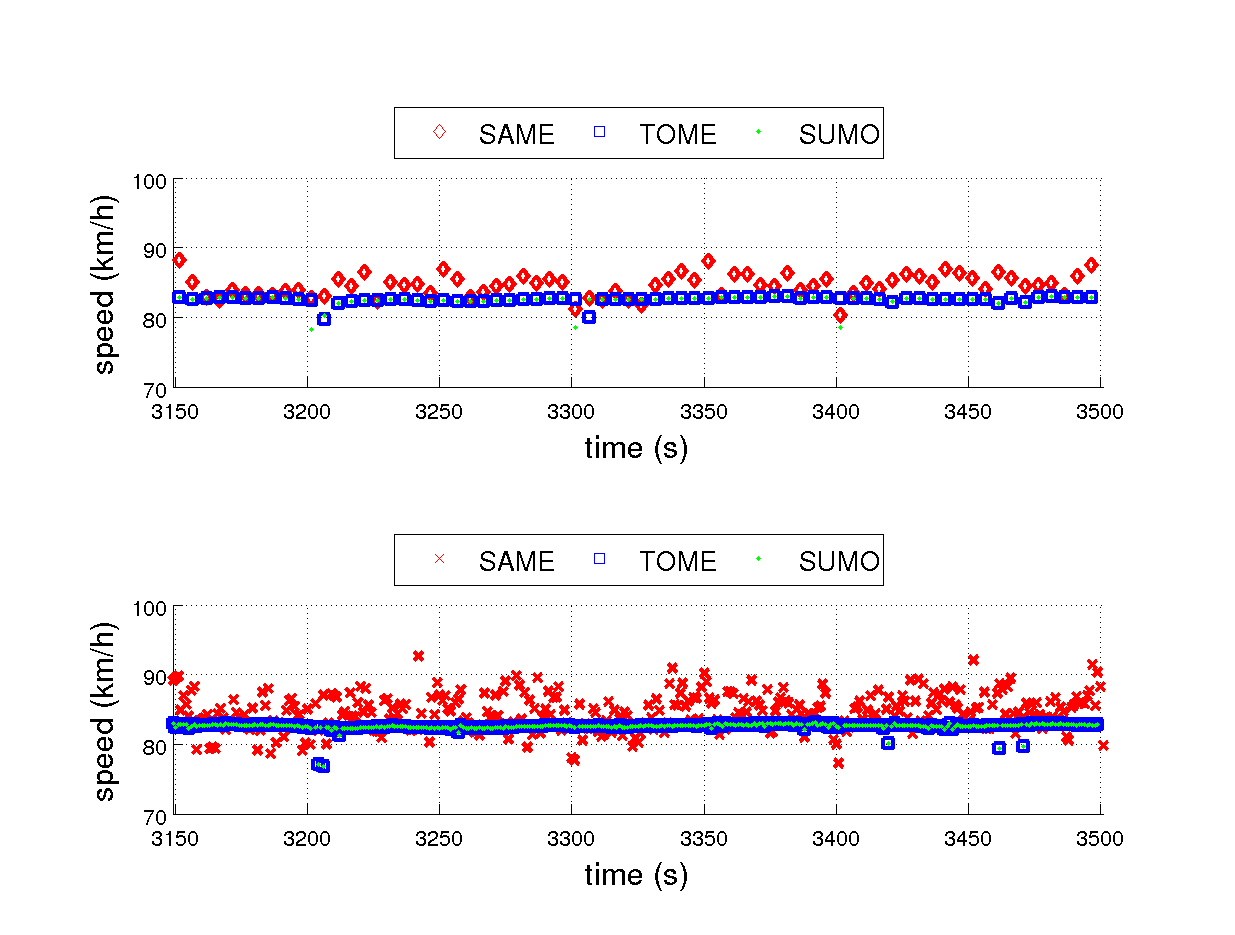
\includegraphics[width=.8\columnwidth]{fig/penetration1.eps}}
\subfigure[75\% of OBU-equipped vehicles, regular traffic conditions]{\label{fig:pen075}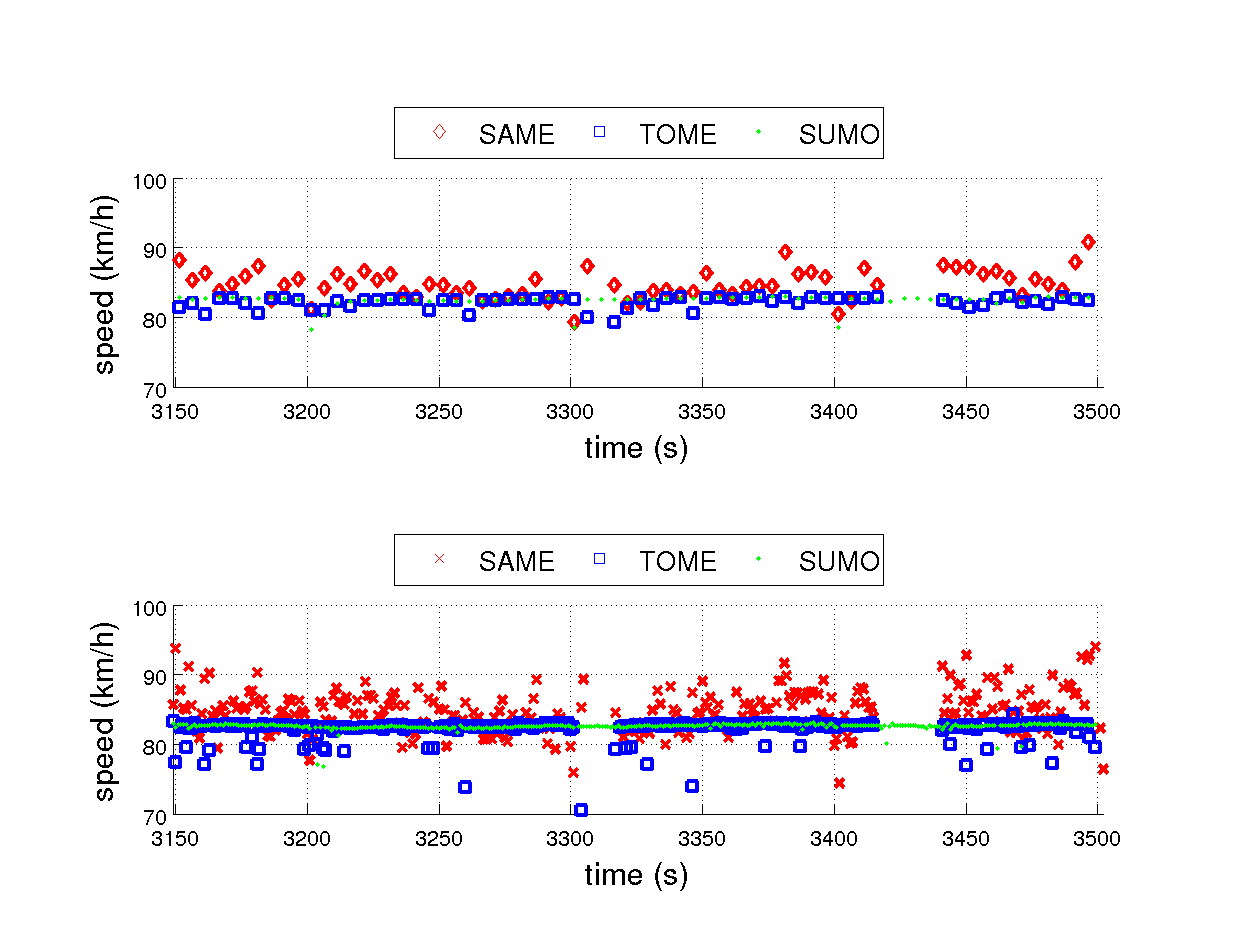
\includegraphics[width=.8\columnwidth]{fig/penetration0.75.eps}}
\subfigure[50\% of OBU-equipped vehicles, regular traffic conditions]{\label{fig:pen05}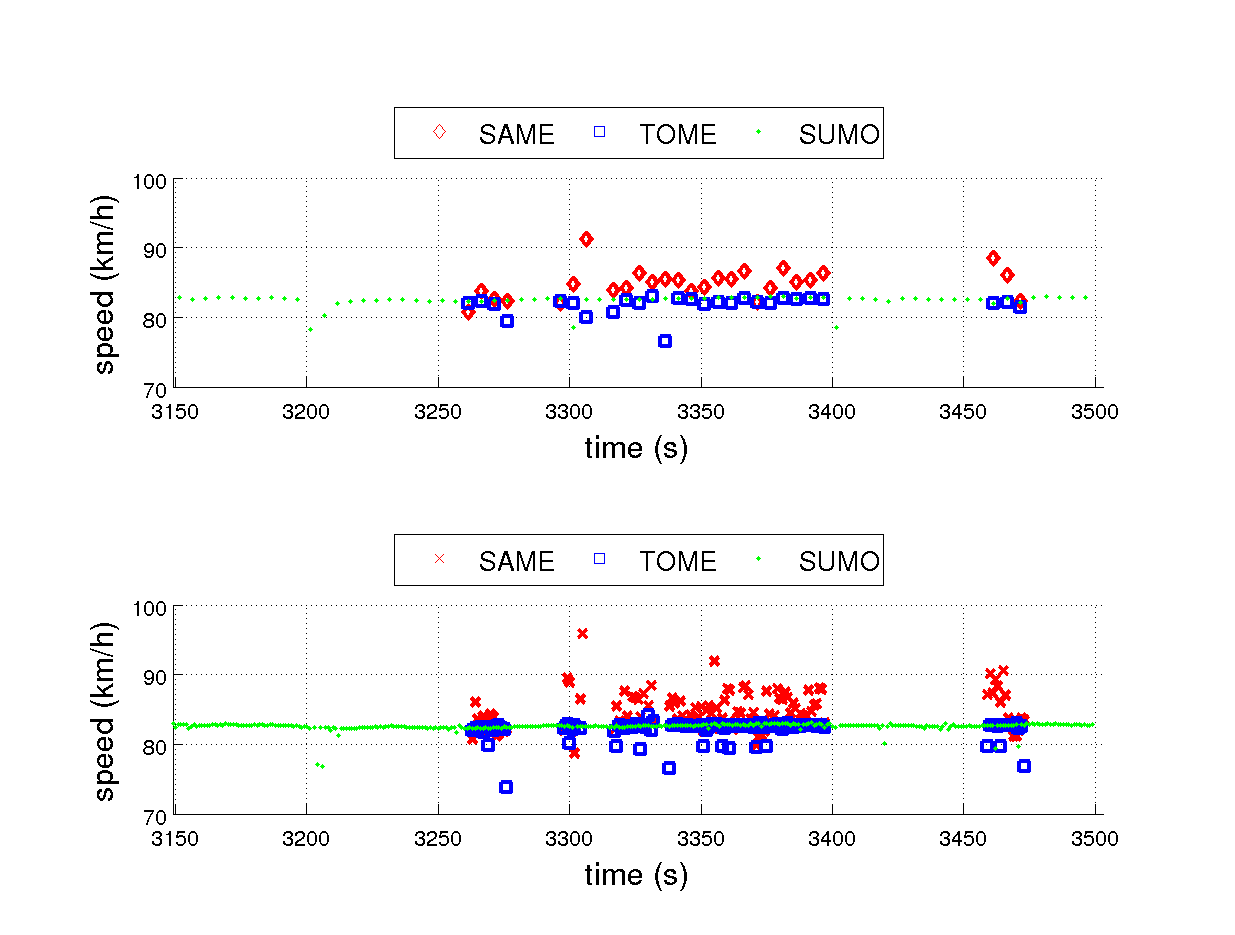
\includegraphics[width=.8\columnwidth]{fig/penetration0.5.eps}}
\subfigure[100\% of OBU-equipped vehicles, incident just before t=2000s]{\label{fig:incid_pen1}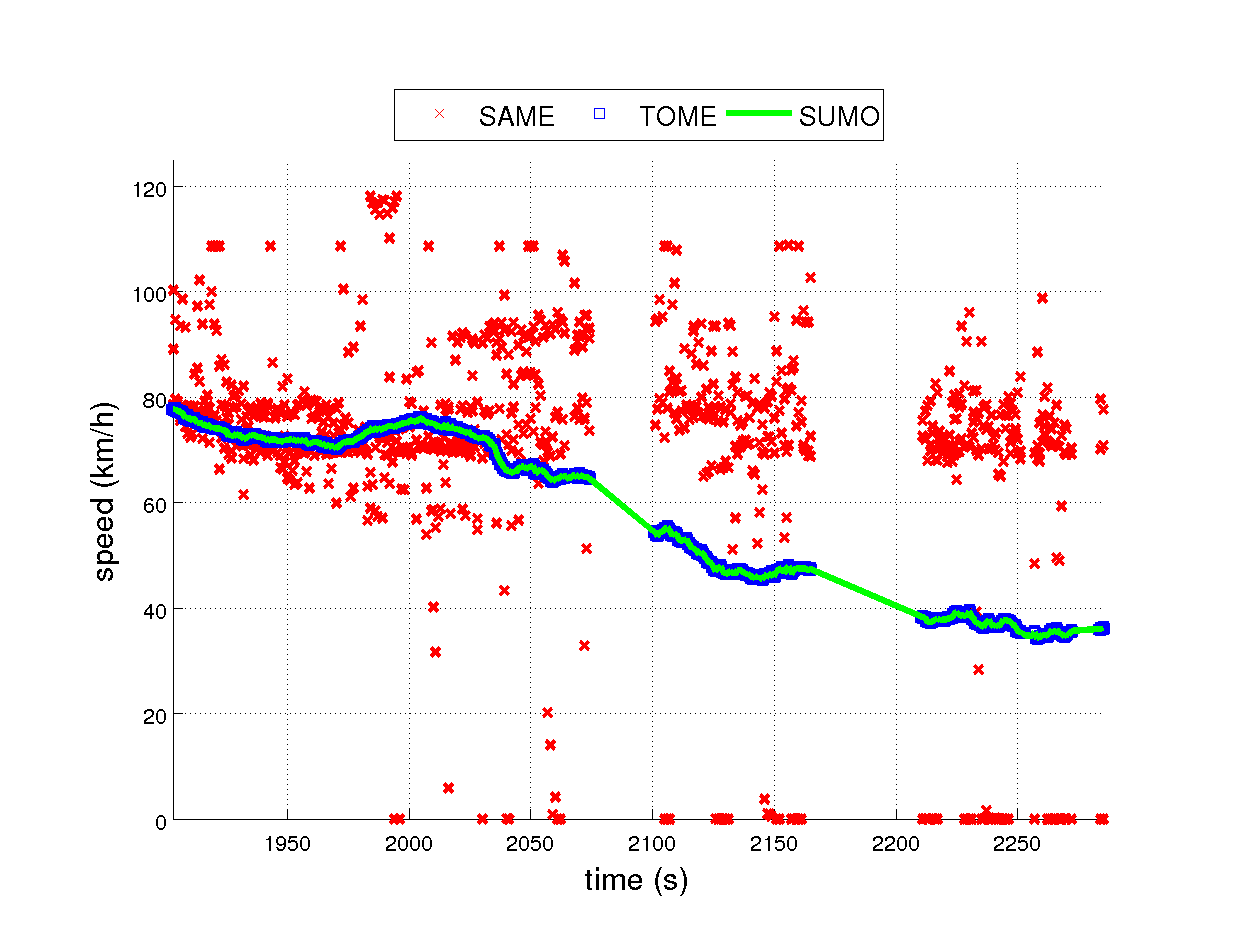
\includegraphics[width=.8\columnwidth]{fig/penetration_incidente_sett141.eps}}
\subfigure[75\% of OBU-equipped vehicles, incident just before t=2000s]{\label{fig:incid_pen075}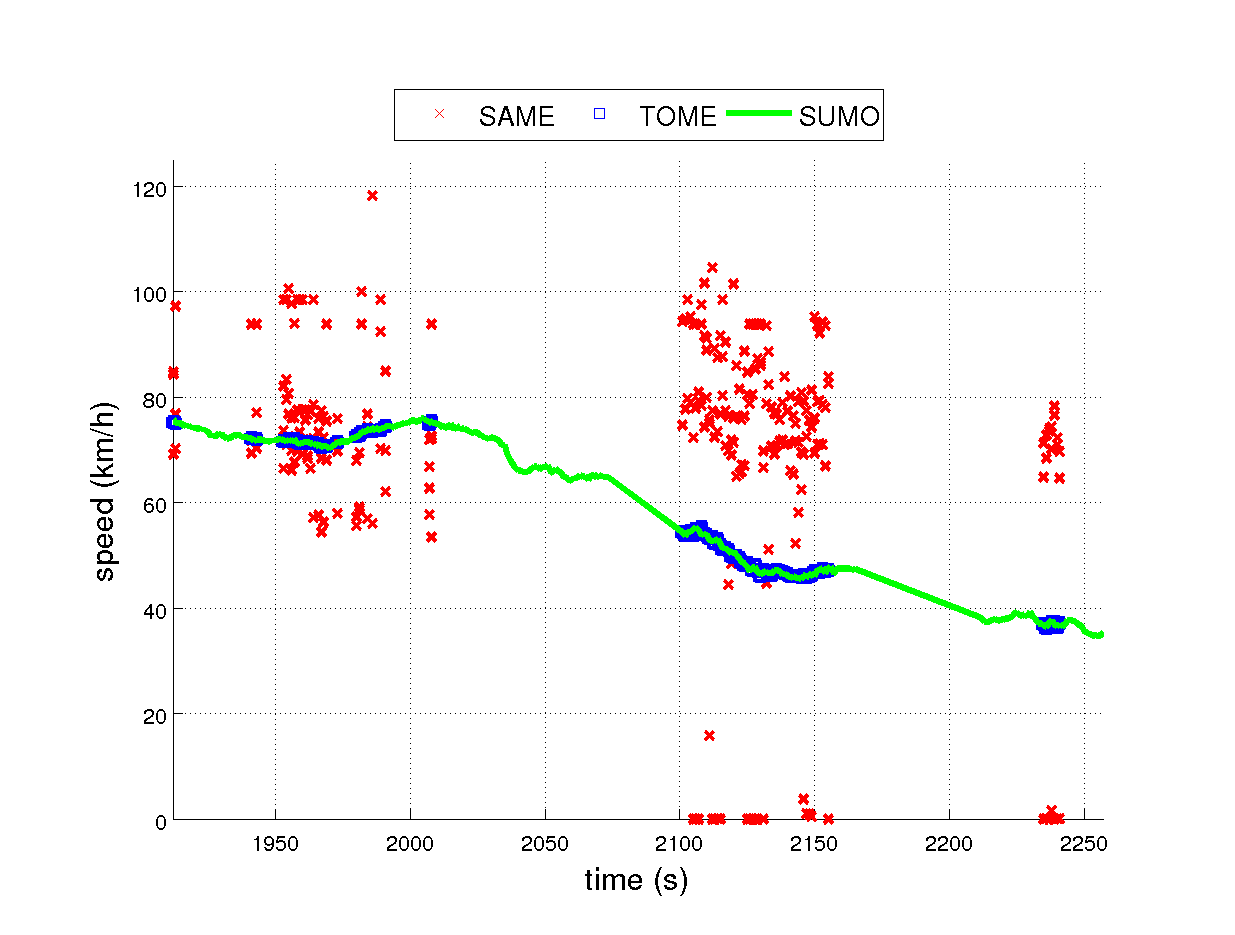
\includegraphics[width=.8\columnwidth]{fig/penetration_incidente_sett140.75.eps}}
\subfigure[50\% of OBU-equipped vehicles, incident just before t=2000s]{\label{fig:incid_pen05}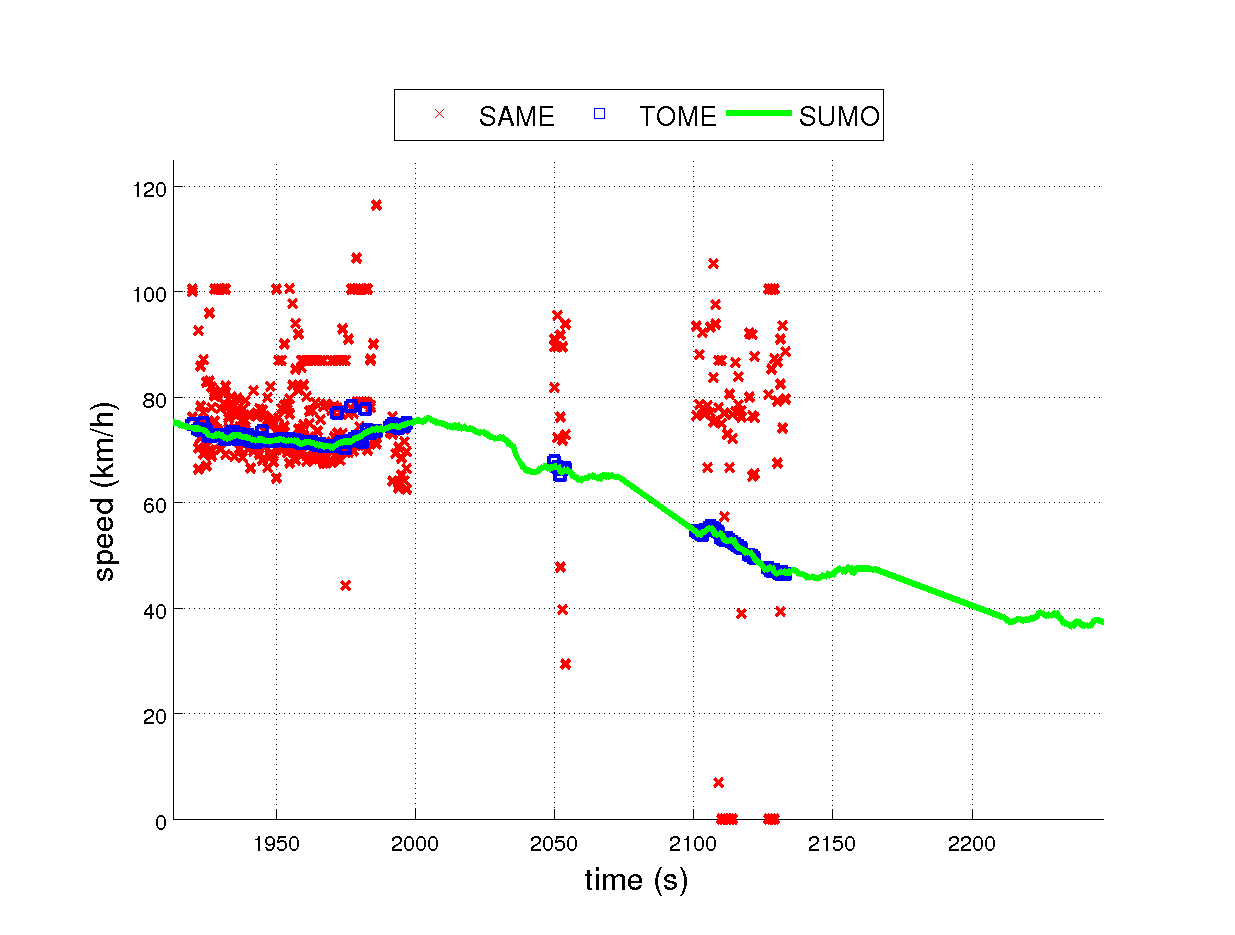
\includegraphics[width=.8\columnwidth]{fig/penetration_incidente_sett140.5.eps}}
\caption{Speed measures on the whole highway, when varying the market penetration rate of the system, in case of regular traffic conditions (a,b,c), with results aggregated every $5~sec$ (on top) and every second (bottom) and speed measures of sector \#14 of the highway in case of incident (d,e,f)}
%\caption{Speed measure when varying the penetration rate of our system. Average every 5s (on top) and every 1s (bottom)}
\label{fig:penetration}
\end{center}
\end{figure*}
By considering the top plots in Figures \ref{fig:pen1}, \ref{fig:pen075} and \ref{fig:pen05}, it is clear that TOME achieves a high accuracy degree in the estimation of the vehicle speed, since it collects speed samples from essentially all vehicles. Remarkably, also SAME turns out to be quite accurate, even though it just samples one vehicle every $R_{max}$, which is one order of magnitude less vehicles than TOME. Overall, the estimate by SAME is based on about 90 samples per round. For the averaging time of $5~sec$, at most about 450 vehicle samples are taken. This is apparently enough to provide an accurate estimation of the average speed in regular traffic conditions. The effect of limited availability of OBU equipment on board vehicles is that some messages get lost due to the temporary disconnection of the VANET chain along the ring highway. The disconnection extent over time grows as the market penetration rate gets smaller. During the presumably long time when VANET equipment is being deployed, heterogeneous networking, exploiting the cellular network should be a solution in order to prevent too frequent disconnections and allow a regular monitoring of the highway. Once OBU spreading overcomes sensitively 50\% of vehicles, VANET alone can start providing a reliable means of collecting measurements. Another means to improve the VANET reliability is to deploy few more RSUs, even if it is reasonable the RSU density shall be much lower than cellular base station density.

These findings are confirmed by the bottom plots in Figures \ref{fig:pen1}, \ref{fig:pen075} and \ref{fig:pen05}, where the same quantities of the top graphs are plotted, except that the average is performed over $1~sec$. It is evident that SAME tends to yield a less stable result than TOME, somewhat overestimating the true average value, but still it keeps the error below 10\% in almost any condition or market penetration rate. Taking into account that we target real time vehicular traffic monitoring, we have to strike a balance between accuracy and delay. From our results, it appears that $5~sec$ can yield a good compromise.

Similar results are obtained by analyzing each highway sector, with more variability for SAME, due to the limited number of samples it collects (few units per sector, a sector being $2.4~km$ long on average).

A last consideration should be said about the required bitrate both for SAME and TOME: in the first case it is almost null (0.08 kbps), which yelds the possibility of a permanent nearly invisible service, running on the control channel or on any non-dedicated sub-channel; in the second case, the bitrate is about 56 kbps, better suited for a channel explicitly dedicated to traffic monitoring services.


%\begin{figure}[tb]
%\begin{center}
%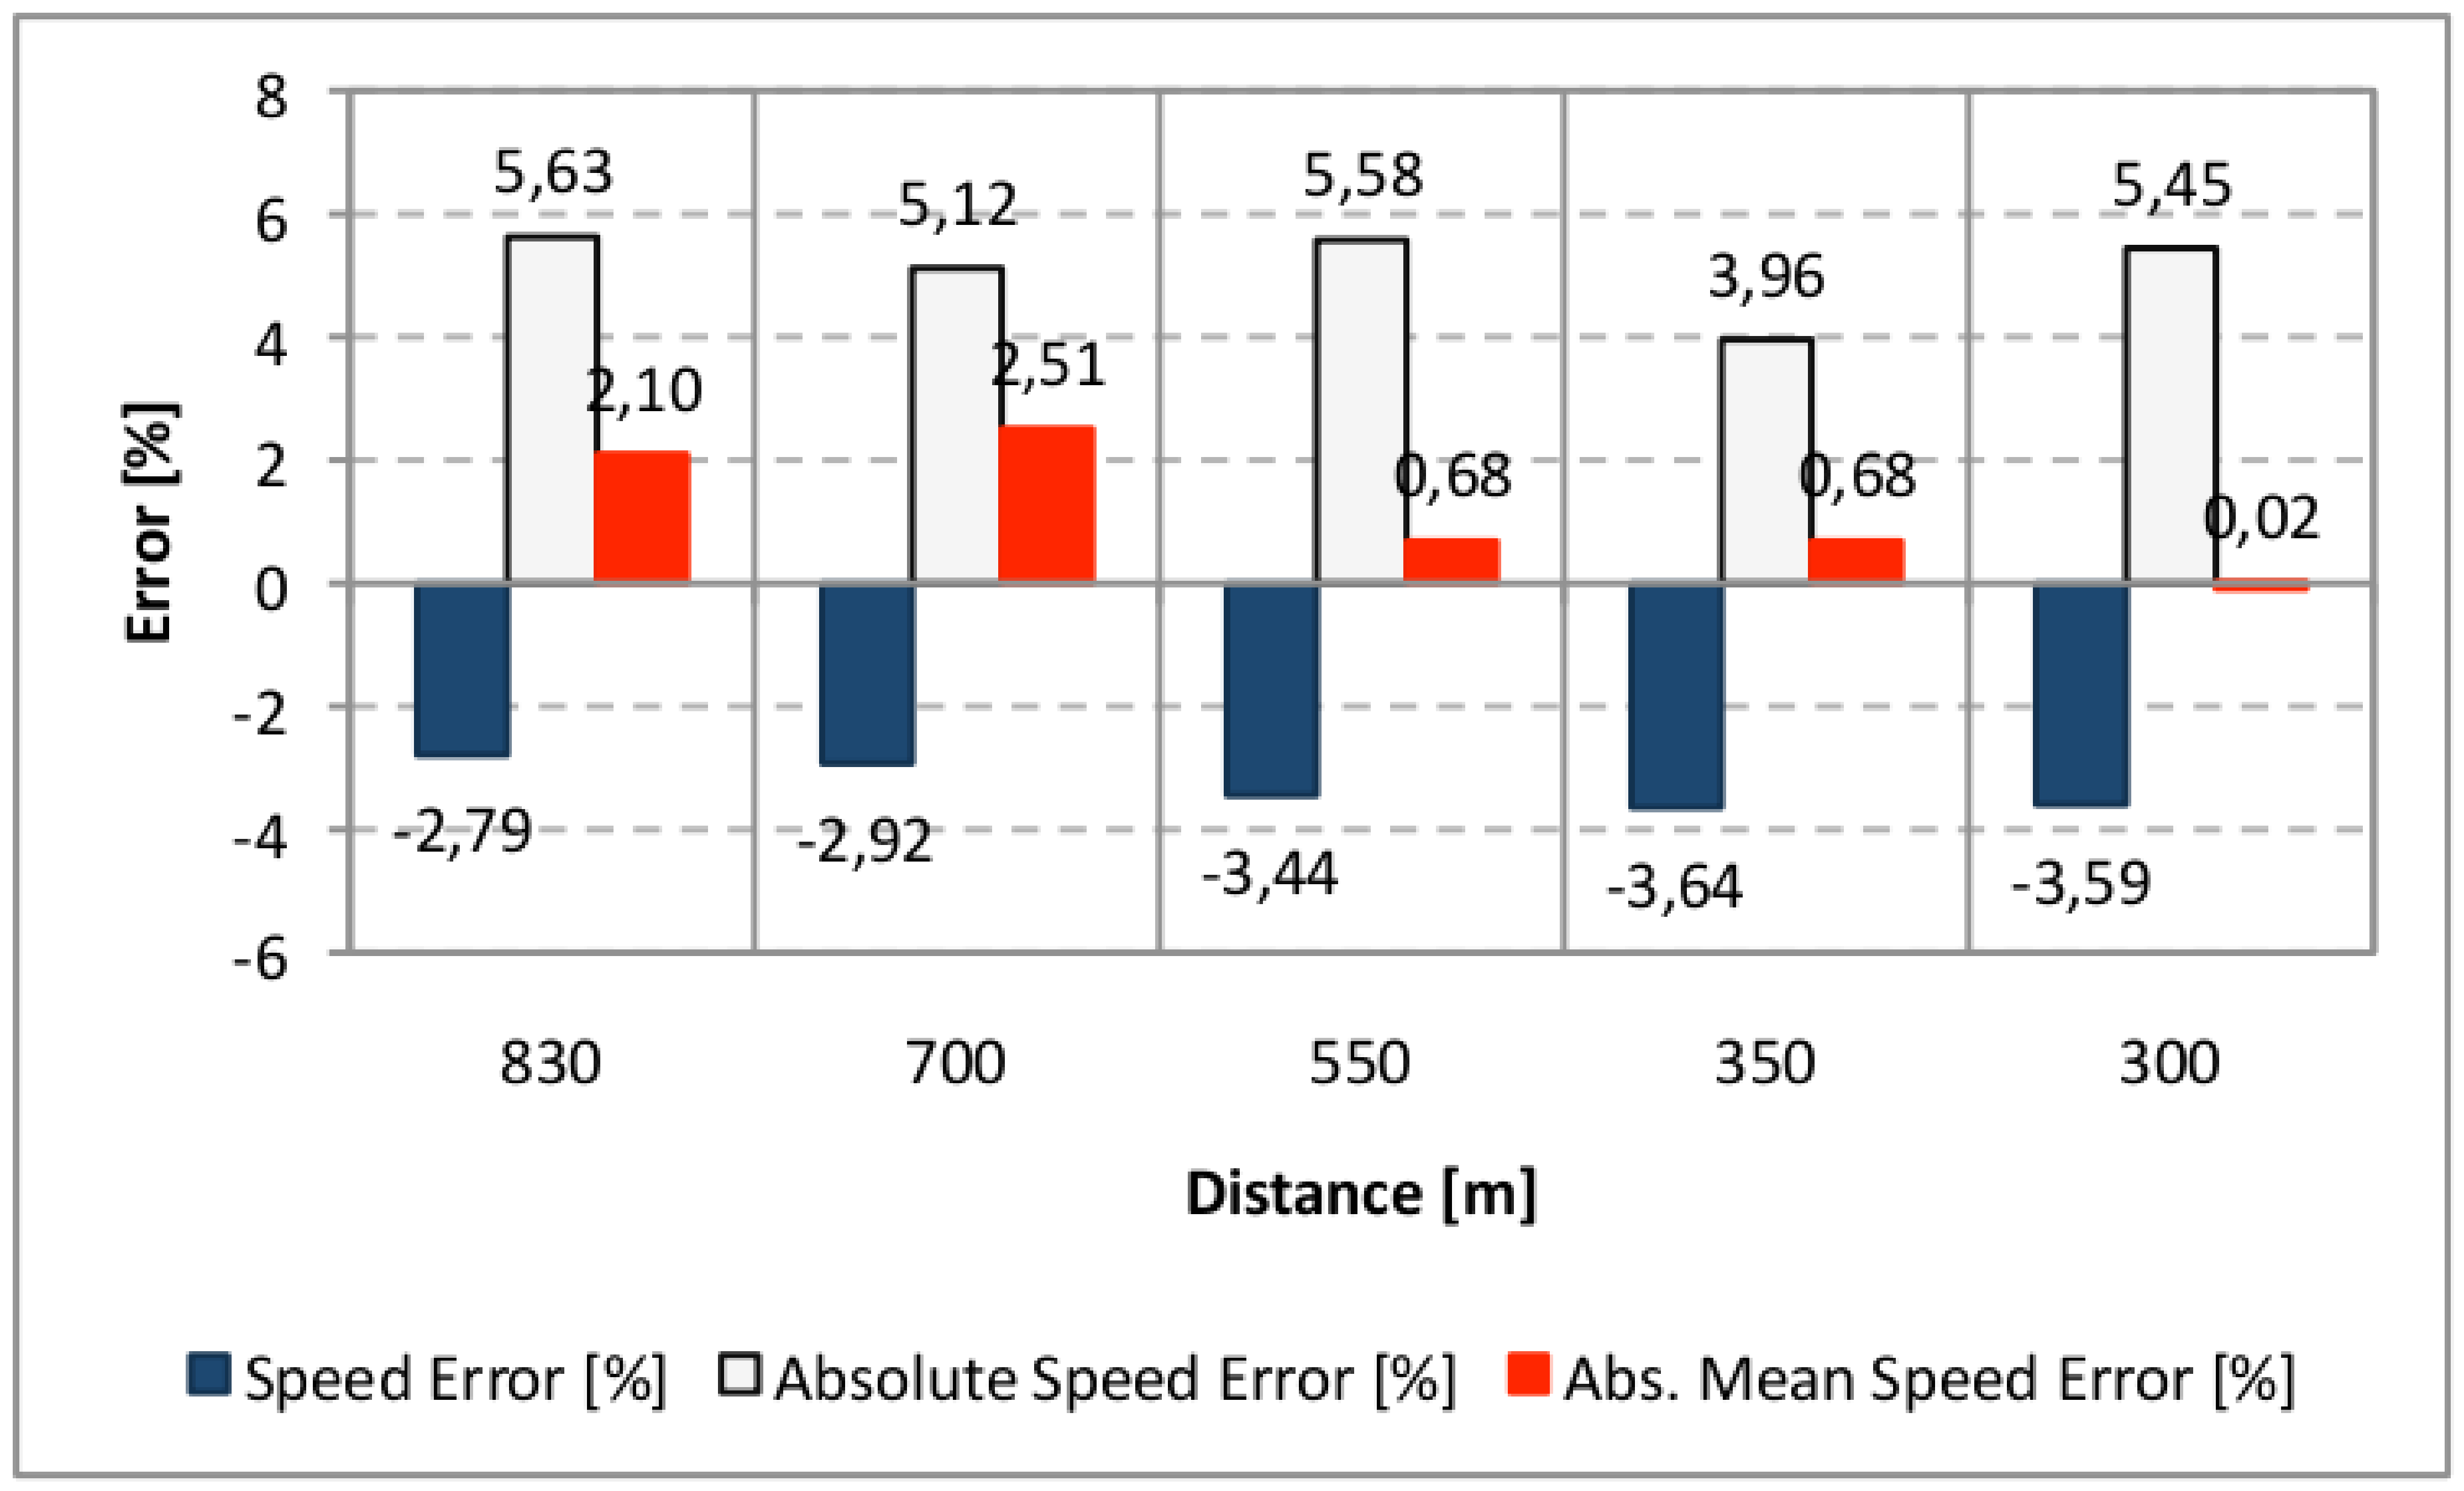
\includegraphics[width=.95\columnwidth]{fig/reliability.eps}
%\caption{Difference from the measures}
%\label{fig:reliability}
%\end{center}
%\end{figure}



\subsection{Incident detection through VANET monitoring}
\label{subsec:stationary}
In this section we analyze the behavior of our protocols when dealing with an incident (Figure \ref{fig:incid_pen1}, \ref{fig:incid_pen075} and \ref{fig:incid_pen05}). These figures refer to only one sector of the GRA, namely sector \#14, that is the one where the incident occurs. Moreover, SAME points are the individual speed samples taken from sampled vehicles within the tagged sector and transported by the protocol.

It is clear that in this case the market penetration rate is a very important factor, since after the accident occurs, the vehicle flow is strongly slowed down and becomes irregular in the interested sector. In terms of communications working, this means that connectivity is not always granted. In fact, even with $p=1$, we have  blank spots in Fig. \ref{fig:incid_pen1}, as for  $2160 < t < 2200~sec$.

By looking at Fig. \ref{fig:incid_pen1}, we get a very clear information about what is going on from SAME. As soon as an incident occurs, immediately we observe two aspects:
\begin{enumerate}
	\item higher variance in the monitored speed.
	\item a sudden increase of (almost) zero speed vehicles.
\end{enumerate}


These two aspects combined together immediately trigger an alarm, detecting the presence of an incident.
The average speed of the vehicles from our ground truth and from TOME, instead, needs some time to drop down, because at the beginning the problem is very localized and the observed sector is 2 Km long, so vehicles that overcome the incident, accelerate and take the same speed they had before they encountered the incident, or even a higher one, because of the reduced density downstream the bottleneck formed by the stopped vehicles. This means that only after $50-100~sec$ TOME really gets aware that an anomaly has occurred (it is possible to notice the descending slope after the incident in the figure).
Moreover, the fact that SAME detects many zero speed values is a clear signal that a stable queue has been formed upstream a sudden bottleneck: this fact identifies an incident. As market penetration rate drops down, the capability to reveal an incident is delayed.
Finally, it is important to notice that SAME takes one order of magnitude less time than TOME to collect and deliver such information (about $4~sec$ vs $41~sec$ respectively).

In order to help showing the SAME capability to reveal an incident, we can automate the incident detection process (e.g., by building an app that automatically yields an alert signal at the traffic monitoring center). The idea is based on the number of zero speed vehicles in a short time frame. Let us define $T_{observation}$, which represents the period of time between a $cmc$ message and the following one. Say that $T_{observation}=1~sec$, and let $z[k]$ be the number of speed samples that fall below a threshold that represents ``blocked'' vehicles at the $k$-th $T_{observation}$ (e.g., we could set a threshold at 10 or 20 km/h). Then, an alert is triggered if the following condition is verified:
$$
e + \sum_{i=k-9}^{k-5} z[i]  < 2 \sum_{ j=k-4 }^{ k } z[j]
$$
where $e$ is a sensibility constant that we set equal to 5, needed to protect the system from false positives when only few vehicles slow down.
This calculation is performed every time a new $cmc$ message is received (thus every $T_{observation}$). By applying this procedure, we can get aware of the incident in $4~sec$ for $p=1$, $103~sec$ for $p=0.75$ and $115~sec$ for $p=0.5$, transmission times included.



\section{NEW PART: to be integrated with the rest}
\label{sec:Scenario}

We simulated a car incident on every sector of our scenario, for a total of 29 sectors, by blocking 2 out of 3 lanes of the highway at a precise time instant (one incident for every simulation). Our SAME protocol is running on the network for monitoring purpose and we measure the car incident detection time as the time that goes from the time instant in which the incident actually takes place to the instant in which the RSU detects the accident; hence all the transmission delays and the observation time to understand that an accident took place (see sec. \ref{sec:detecting}) are already included.





\section{Performance Evaluation}
\label{sec:performance}

In Fig. \ref{fig:code}, we plotted the queue length directly from the SUMO simulation output, over the 2 lanes blocked by the car incident, as a result of the average queue length detected on every simulation, on the congested sector. We also plotted the incident notification time of our scheme, SAME, for the different market penetration rates, defined in sec. \ref{sec:Scenario} in relation to the queue maturated on the road segment.

As we can see, Lane 0, which is the slowest lane on the right, has a very constant que grow rate, since most of the vehicles that arrive at the incident location just brake and enqueue behind the other ones. Lane 1, instead, has a different behavior, since after a first phase (from $t=0$ to $t \approx 120$) where it grows just like Lane 0, then it starts being more inconstant, with faster increases and decreases, since vehicles try to overcome the incident by choosing the third lane on the left, which is free from the accident, but still used by the vehicles that flow on the road from behind. With a visual simulation inspection, this translates into watching vehicles that try to depart from Lane 1 to Lane 2 to overcome the incident and the blocked portion of the road.

It is very interesting to notice that SAME can actually inform the RSU of the incident when the que is no more bigger than 25-30 m, which is a very interesting result, since this value can be granted also when the market penetration rate falls from 100\% to 75\%. Even when such market penetration rate value falls down to 50\% of the vehicles equipped with this technology, the line does not exceed 70m per lane on the average.

This means that an accident can be detected and a reaction can be triggered when its consequences are still at a very early stage, before that the situation degenerates into a huge traffic jam.

In Fig. \ref{fig:rilevazione_incidenti}, instead, we evaluate the distribution of the incident detection time, grouped by 20s time windows. Again, we obtained those results as an average computed on the results of all the simulations on the different road segments where we simulated the incident.

It appears a clear and encouraging distribution pattern for all the market penetration rates. In particular, in Fig. \ref{fig:rilevazione1}, where it is equal to 100\%, we show that more of the 50\% of all the incidents are detected by the RSU within the first 20s after the accident actually happens and if we wait for 40s, about 80\% of the accidents are revealed and reported. Again, this means that in combination with the results of Fig. \ref{fig:code}, within 20s and a 25m queue on the average, a reaction can be triggered, like sending  emergency vehicles on the place and redirecting the traffic over other routes.
When the market penetration rate decreases to 75\% (Fig. \ref{fig:rilevazione0.75}, we still observe a very good reactivity of our system to the obstruction. In fact, in this case, within 40s about 75\% of the accidents are revealed and reported, with the same detection time trend observed in Fig. \ref{fig:rilevazione1}. What makes this case different with respect to the previous one is that the notification is more spread over time: in some cases it may take up to 100s.

This happens because when the market penetration rate drops down, only few vehicles can overtake the accident, especially in the first time instants after the problem occurred. This means that there may be an occasional hole in the vehicles distribution, such that the wireless multi-hop chain breaks and the information cannot travel over the whole ring and reach the RSU back (notice that in this case, the other travel direction is not used to relay packets).
The lesser the market penetration rate, the greater the probability that this event occurres, as we can see in Fig. \ref{fig:rilevazione0.5}, where the market penetration rate is 50\%. In this case, in fact, there is no detection before 40s and only after that time frame we can observe a distribution which is similar to the previous cases.




\begin{figure}[tbhp]
\begin{center}
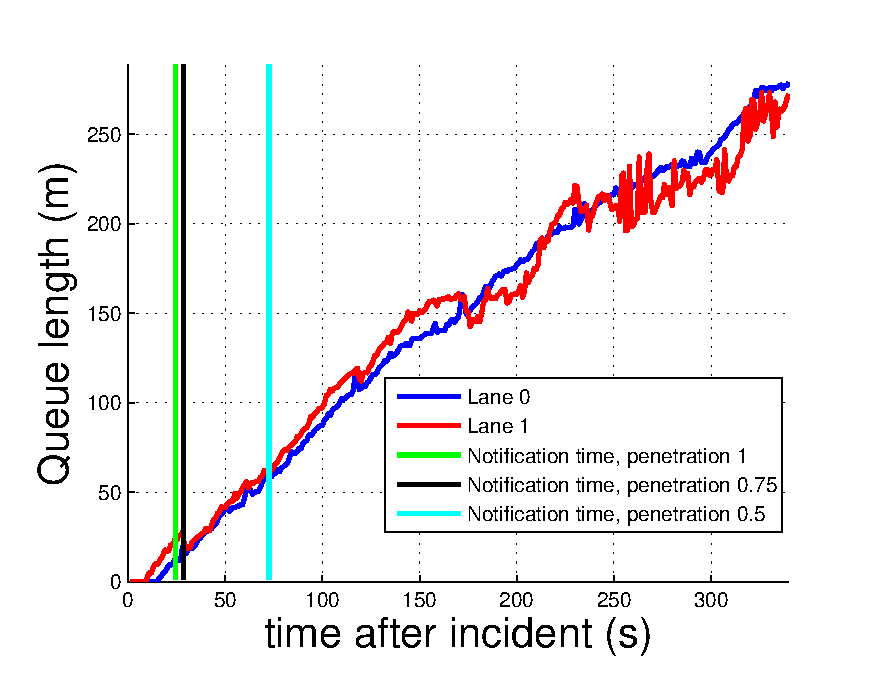
\includegraphics[width=.8\columnwidth]{./fig/stampa_code.eps}
\caption{Average queue length for both the lanes blocked by the accident. The vertical lines display the algorithm  notification time as a function of the DSRC market penetration rate}
\label{fig:code}
\end{center}
\end{figure}

\begin{figure}[!t]
	\begin{center}
    \subfigure[Penetration Rate=100\%]{\label{fig:rilevazione1}\includegraphics[width=.8\columnwidth]
        {./fig/stampa_rilevazioni_incidente_tempi_medi1.eps}}
    \subfigure[Penetration Rate=75\%]{\label{fig:rilevazione0.75}\includegraphics[width=.8\columnwidth]
        {./fig/stampa_rilevazioni_incidente_tempi_medi0.75.eps}}
\subfigure[Penetration Rate=50\%]{\label{fig:rilevazione0.5}\includegraphics[width=.8\columnwidth]
        {./fig/stampa_rilevazioni_incidente_tempi_medi0.5.eps}}
	\caption{Percentage of accidents detected in 20s time windows, by considering several market penetration rate values}
	\label{fig:rilevazione_incidenti}
	\end{center}
\end{figure}



\bibliographystyle{IEEEtran}
\bibliography{biblio}


\end{document}
